% !TEX root = documentacao.tex
\chapter{Documentação do usuário}

Esta parte da documentação é destinada a usuários do código e foi subdividida
em tutoriais. Estes tutoriais tem como objetivo familiarizar o usuário
com os comandos utilizados no código, começando por exemplos bem simples até os
casos mais complexos. Cada tutorial é acompanhado de um código executável.Para compilá-los individualmente, basta usar o comando \texttt{make nome\_do\_tutorial DIM=dim\_do\_tutorial} (\texttt{nome\_do\_tutorial} não inclui o \texttt{.c}). Para compilar todos de uma só vez, usa-se \texttt{make all}.

%%%%%%%%%%%%%%%%%%%%%%%%%%%%%%%%%%%%%%%%%%%%%%%%%%%%%%%%%%%%%%%%%%%%%%%%%%%%%%%%%%%%%%%%%%%
%%%%%%%%%%%%%%%%%%%%%%%%%%%%%%%%%%%%%%%%%%%%%%%%%%%%%%%%%%%%%%%%%%%%%%%%%%%%%%%%%%%%%%%%%%%

\section{Tutorial 1 -- Gerando uma malha 2D}

Nesta seção iremos gerar uma malha bidimensional, em um domínio retangular,
o qual damos o nome de {\it root}, e subdividi-lo em células. Esta
será a malha raiz e a partir dela poder-se-á
refiná-la nas regiões aonde o usuário achar conveniente.  Iniciamos com uma
malha bidimensional, portanto onde referencia-se a variavel {\it DIM}, ela terá valor 2.
O código completo se encontra no
diretório {\it tutoriais}, com o nome de {\it tutorial01-2d.c}. A seguir será descrito o
que é realizado em cada comando do código.

Primeiramente é necessário incluir as definições minimamente necessárias para a execução do código, as bibliotecas padrão do sistema e da HiG-Tree:
\begin{verbatim}
#include<stdio.h>
#include<stdlib.h>
#include "higtree.h"
#include "higtree-io.h"
\end{verbatim}
A seguir, inicializa-se o bloco principal
\begin{verbatim}
int main(int argc, char *argv[])
\end{verbatim}
A malha será gerada em um retângulo, desta forma é necessário declarar então os pontos inferior esquerdo {\it lp} e superior direito {\it hp}, além de atribuí-los um valor
\begin{verbatim}
Point lp, hp;
POINT_ASSIGN_SCALAR(lp, -1.0);
POINT_ASSIGN_SCALAR(hp,  1.0);
\end{verbatim}
Veja que neste caso atribuimos $ lp=(-1,-1)$ e $ hp=(1,1)$ através da macro \verb|POINT_ASSIGN_SCALAR|, que substitui o código
\begin{verbatim}
lp[0] = -1.0;
lp[1] = -1.0;
hp[0] =  1.0;
hp[1] =  1.0;
\end{verbatim}
Com os pontos $lp$ e $hp$ declarados, basta criar a malha com o comando
\begin{verbatim}
hig_cell *root = hig_create_root(lp, hp);
\end{verbatim}

Com este comando, a célula endereçada pela variável {\it root} foi criada. Agora é necessário subdividi-la em uma malha regular. Para este exemplo, vamos gerar uma malha de $2\times 2$ elementos. Primeiro, declara-se o número de células desejadas em cada direção (lembrando que {\it DIM=2})
\begin{verbatim}
	int num_cell[DIM];
	POINT_ASSIGN_SCALAR(num_cell, 2);
\end{verbatim}
e invocar o comando
\begin{verbatim}
	hig_refine_uniform(root, num_cell);
\end{verbatim}
para criar a malha desejada.

Para visualizar a malha, basta criar um arquivo {\it vtk} e imprimir a malha  no arquivo. Isto pode ser realizado da seguinte forma:
\begin{verbatim}
	FILE *fd = fopen("VTKS/tut01.vtk", "w");
	higio_print_in_vtk2d(fd, root);
	fclose(fd);
\end{verbatim}
Uma imagem da malha gerada pode ser vista na figura \ref{fig:tutorial_malha_1}.

\begin{figure}
	\centering
	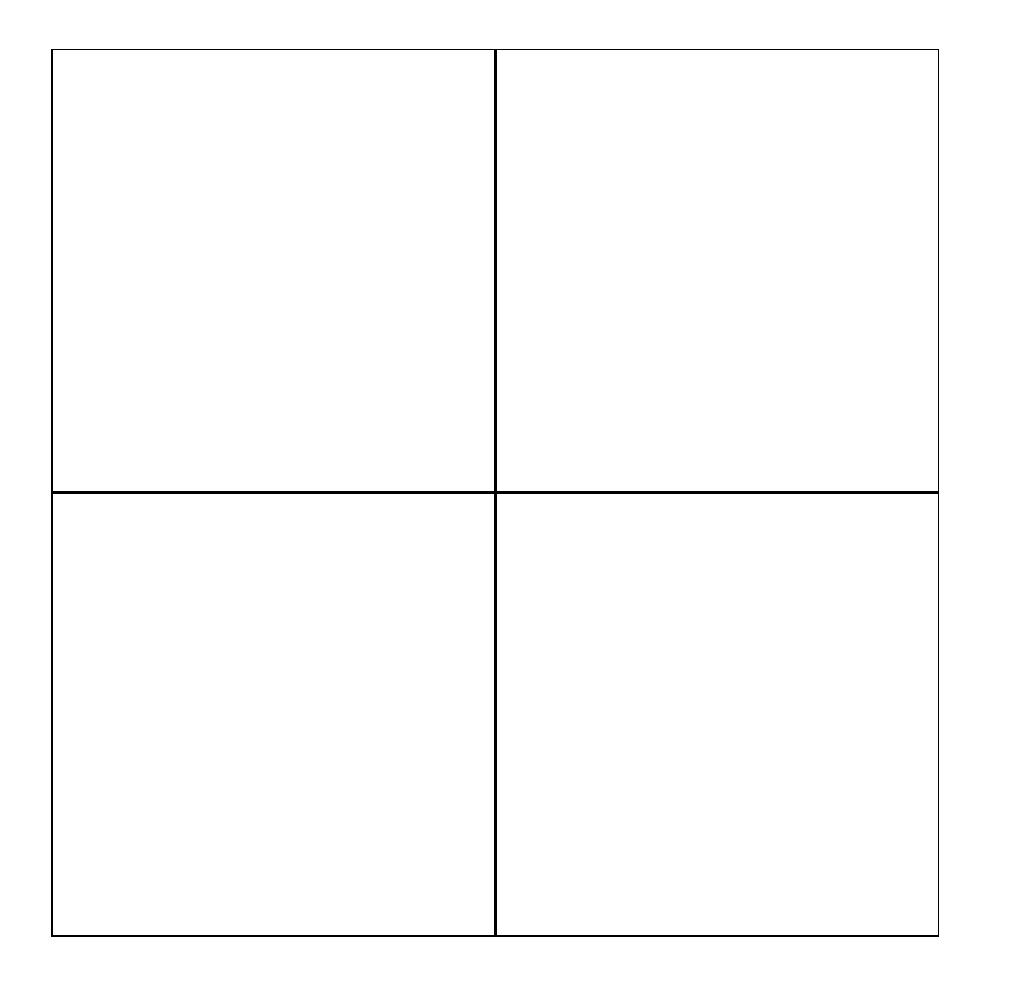
\includegraphics[width=0.6\linewidth]{figuras/tutorial_malha_1.png}
	\caption{Malha gerada pelo tutorial 1.}
	\label{fig:tutorial_malha_1}
\end{figure}

Após realizados todos os cálculos a raiz tem que ser destruída para não ficar ocupando
espaço em memória, o que é feito através do comando:
\begin{verbatim}
	hig_destroy(root);
\end{verbatim}


%%%%%%%%%%%%%%%%%%%%%%%%%%%%%%%%%%%%%%%%%%%%%%%%%%%%%%%%%%%%%%%%%%%%%%%%%%%%%%%%%%%%%%%%%%%
%%%%%%%%%%%%%%%%%%%%%%%%%%%%%%%%%%%%%%%%%%%%%%%%%%%%%%%%%%%%%%%%%%%%%%%%%%%%%%%%%%%%%%%%%%%

\section{Tutorial 2 -- Refinamento de células}
\label{sec:tut2}
Nesta seção iremos tomar uma malha bidimensional gerada como no exemplo
anterior, mas com 4 células na direção $x$ e 5 na direção $y$, e realizar o
procedimento de refinamento, ou seja, tomar uma ou mais células da malha e
dividi-la em partes menores. O código a ser adotado se encontra no diretório
{\it tutoriais}, com o nome de {\it tutorial02-2d.c}. A seguir será descrito o que é
realizado em cada comando do código.

Após inicializada a nova malha, subdivide-se o domínio da forma descrita acima
\begin{verbatim}
	int num_cell[DIM];
	num_cell[0] = 4;
	num_cell[1] = 5;
	hig_refine_uniform(root, num_cell);
\end{verbatim}
Digamos que seja necessário o refinamento de células próximo ao ponto $(0.5,0.5)$. Definamos o ponto $p$
\begin{verbatim}
	Point p;
	p[0] = 0.5;
	p[1] = 0.5;
\end{verbatim}
Em seguida, selecionamos a célula a ser refinada através do comando
\begin{verbatim}
	hig_cell *c = hig_get_cell_with_point(root,p);
\end{verbatim}
Para realizar o refinamento da célula que contém o ponto {\it p},
define-se o número de células que será utilizado para este refinamento nas duas
direções e em seguida é dado o comando de refinamento uniforme na célula {\it
c}.
\begin{verbatim}
	num_cells[0] = 2;
	num_cells[1] = 2;
	hig_refine_uniform(c,num_cells);
\end{verbatim}

Como feito anteriormente, a malha pode ser impressa em arquivo {\it vtk} da seguinte forma
\begin{verbatim}
	FILE *fd = fopen("VTKS/tut02.vtk", "w");
	higio_print_in_vtk2d(fd, root);
	fclose(fd);
\end{verbatim}
A malha resultante pode ser vista na figura \ref{fig:tutorial_malha_2}.

\begin{figure}
	\centering
	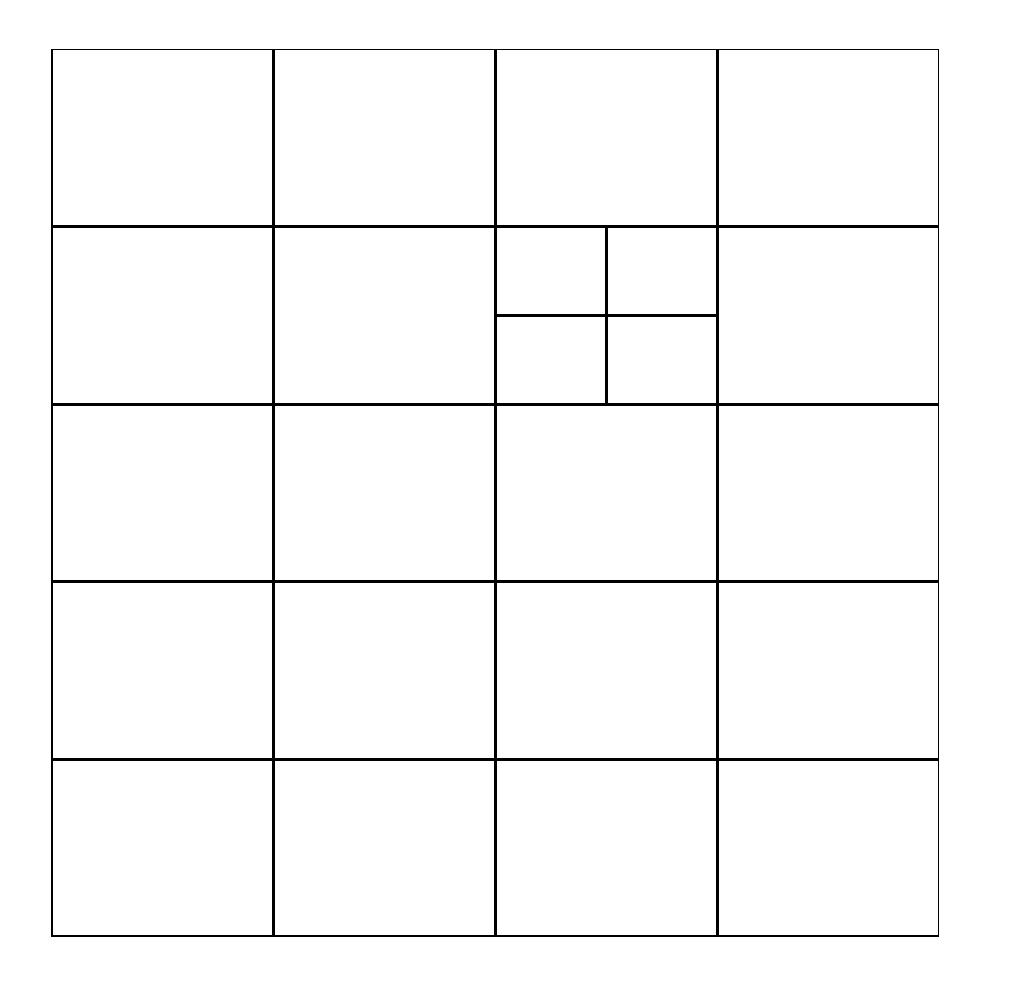
\includegraphics[width=0.6\linewidth]{figuras/tutorial_malha_2.png}
	\caption{Malha gerada pelo tutorial 2.}
	\label{fig:tutorial_malha_2}
\end{figure}



\subsection{Selecionando células através de janelas -- 2D}

%%%%%%%%%%%%%%%%%%%%%%%%%%%%%%%%%%%%%%%%%%%%%%%%%%%%%%%%%%%%%%%%%%%%%%%%%%%%%%%%%%%%%%%%%%
%%%%%%%%%%%%%%%%%%%%%%%%%%%%%%%%%%%%%%%%%%%%%%%%%%%%%%%%%%%%%%%%%%%%%%%%%%%%%%%%%%%%%%%%%%

\section{Tutorial 3 - DIM = 3}

Nesta seção, faremos uma malha tridimensional. O procedimento é análogo ao de criar uma bidimensional, como na seção \ref{sec:tut2}, com a única diferença que temos mais uma coordenada de liberdade para refinar. O código, do arquivo \textit{tutorial03-2d.c}, segue da seguinte maneira:

\begin{verbatim}
	Point lo, hi;
    POINT_ASSIGN_SCALAR(lo, -1.0);
	POINT_ASSIGN_SCALAR(hi, 1.0);
\end{verbatim}
Criamos $lo = (-1.0, -1.0, -1.0)$ e $hi = (1.0, 1.0, 1.0)$ os pontos que definem o paralelepídeo do domínio. O macro \texttt{POINT\_ASSIGN\_SCALAR} coloca o mesmo valor em todas as entradas do vetor.
\begin{verbatim}
	hig_cell *root = hig_create_root(lo, hi); 
	int nc[3] = {2,3,4}; 
    hig_refine_uniform(root, nc);
\end{verbatim}

Criamos a célula e então a refinamos com $2$ células na direção $x$, $3$ na direção $y$ e $4$ na direção $z$.

\begin{verbatim}
	Point a;
    POINT_ASSIGN_SCALAR(a, 0.5);
    hig_cell *c = hig_get_cell_with_point(root, a);
    nc[0] = 2; nc[1] = 2; nc[2] = 2;
    hig_refine_uniform(c, nc);
\end{verbatim}

Pegamos a célula com o ponto $a = (0.5, 0.5, 0.5)$ e a refinamos com em 8 células distintas ($2\times 2 \times 2$).

\begin{verbatim}
	FILE *f = fopen("VTKS/tut03.vtk", "w");
    higio_print_in_vtk3d(f, root);

    fclose(f);
    hig_destroy(c);
\end{verbatim}

Por fim, como feito anteriormente, salvamos a célula criada e finalizamos o programa.

A malha gerada pode ser vista na figura \ref{fig:tutorial_malha_3}:

\begin{figure}
	\centering
	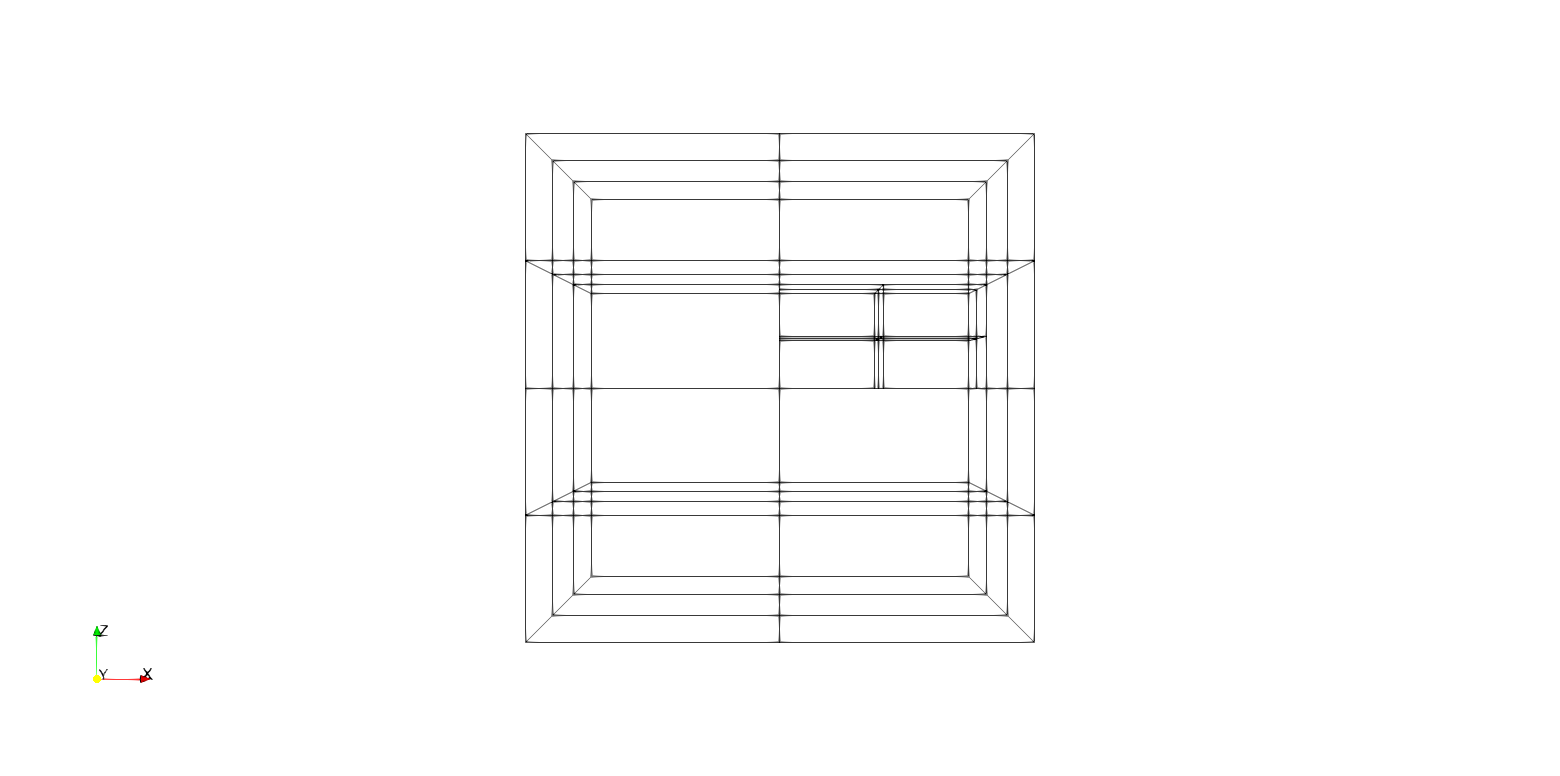
\includegraphics[width=0.9\linewidth]{figuras/tutorial_malha_3.png}
	\caption{Malha gerada pelo tutorial 3}
	\label{fig:tutorial_malha_3}
\end{figure}

%%%%%%%%%%%%%%%%%%%%%%%%%%%%%%%%%%%%%%%%%%%%%%%%%%%%%%%%%%%%%%%%%%%%%%%%%%%%%%%%%%%%%%%%%%
%%%%%%%%%%%%%%%%%%%%%%%%%%%%%%%%%%%%%%%%%%%%%%%%%%%%%%%%%%%%%%%%%%%%%%%%%%%%%%%%%%%%%%%%%%

\section{Tutorial 4 - Usando iteradores}

Este código introduz o uso de iteradores para percorrer as faces ou as células de uma HiG-Tree. Existem dois tipos de iteradores: \textit{higcit\_celliterator} e \textit{higfit\_facetiterator}. Como seus nomes indicam, esses objetos iteram células e faces respectivamente. O código implementado em \textit{tutorial04-2d.c} segue:
\begin{verbatim}
#include "higtree-iterator.h"
\end{verbatim}

Devemos incluir a biblioteca que contém a estrutura e os métodos dos iteradores, além das bibliotecas já mencionadas anteriormente.

\begin{verbatim}
	Point lo, hi;
    POINT_ASSIGN_SCALAR(lo, -1.0);
    POINT_ASSIGN_SCALAR(hi, 1.0);

    hig_cell *root = hig_create_root(lo, hi);

    int nc[2] = {2,2};
    hig_refine_uniform(root, nc);

    Point refine_point;
    POINT_ASSIGN_SCALAR(refine_point, 0.5);
    hig_cell *c = hig_get_cell_with_point(root, refine_point);
    hig_refine_uniform(c, nc);
    FILE *fd = fopen("VTKS/tut04.vtk", "w");
    higio_print_in_vtk2d(fd, root);
    fclose(fd);
\end{verbatim}

Criamos a HiG-Tree da figura \ref{fig:tutorial_malha_4}, O código é análogo aos tutoriais anteriores.

\begin{figure}
	\centering
	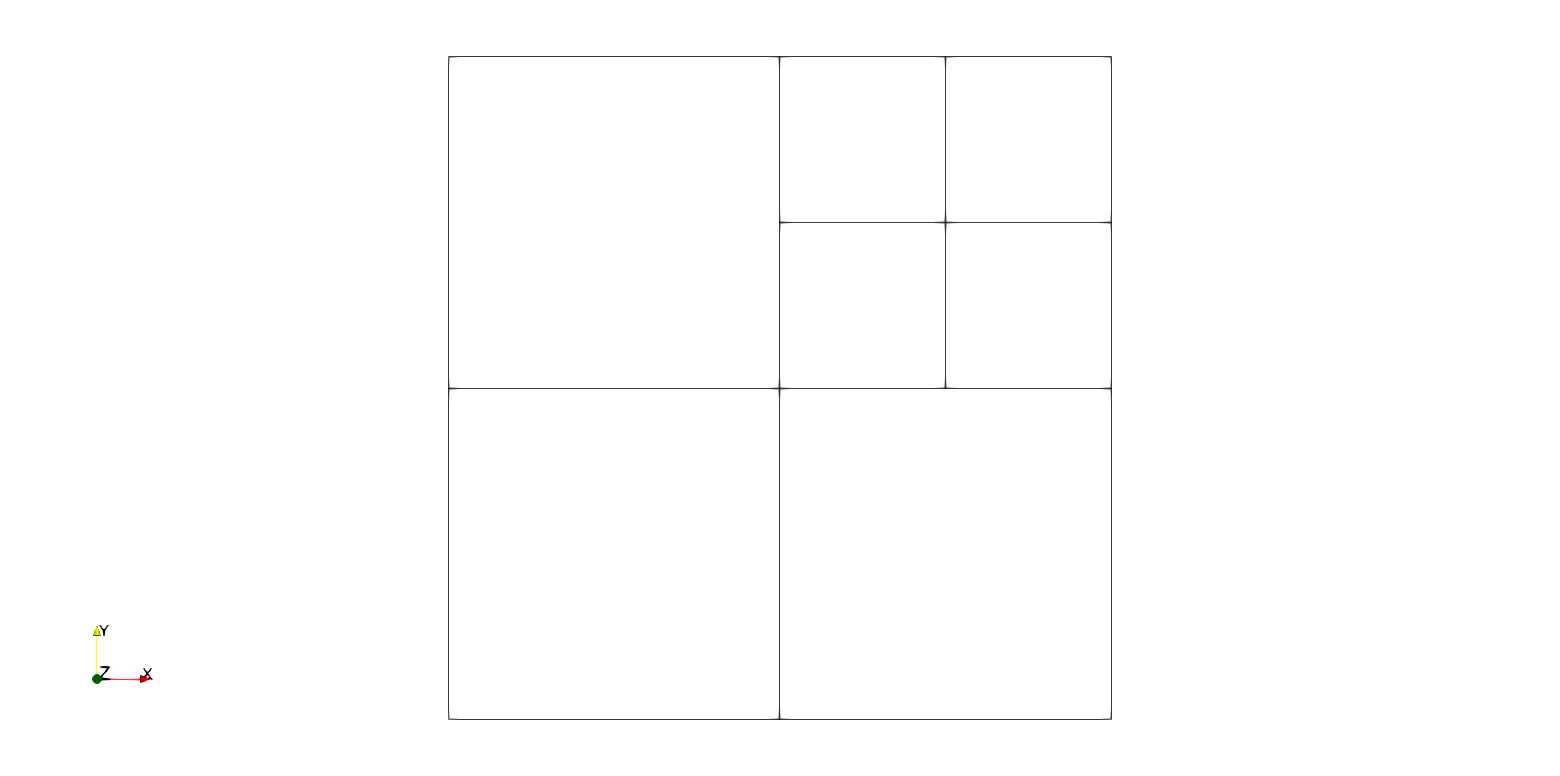
\includegraphics[width=0.9\linewidth]{figuras/tutorial_malha_4.png}
	\caption{Malha gerada no tutorial 4}
	\label{fig:tutorial_malha_4}
\end{figure}

Agora com a célula raíz criada, podemos iterar sobre as células filho. Existem algumas formas de criar um iterador para células, sendo a mais comum (e utilizada nesse tutorial) iterar sobre todas as folhas da árvore (todas as células atuais).
\begin{verbatim}
	higcit_celliterator *cit;
    printf("centers of the cells:\n");

    for(cit = higcit_create_all_leaves(root); 
	!higcit_isfinished(cit); higcit_nextcell(cit)) {
        hig_cell *ccell = higcit_getcell(cit); 
        Point center;
        hig_get_center(ccell, center);
        int id = hig_get_cid(ccell);
        printf("cell: %d \t(x= %.2f, y= %.2f)\n", 
		id, center[0], center[1]);
    }
    higcit_destroy(cit);
\end{verbatim}

Nessa parte apenas iteramos sobre todas as células e imprimimos no terminal o id e a localização do centro da célula. Na primeira linha, declaramos o iterador. Nos argumentos do \texttt{for}, a função \texttt{higcit\_isfinished()} será sempre a condição de parada de um iterador de células e a função \texttt{higcit\_nextcell()} funciona como incremento. A criação do iterador (e a definição de sobre quais células ele irá iterar) acontece com a função \texttt{higcit\_create\_all\_leaves()}. 

Existe uma série de funções \texttt{higcit\_create\_...()} e outras formas de criar iteradores (relacionadas com domínios, serão comentadas nos próximos tutoriais). O leitor é encorajado a procurar sobre essas funções no header file da biblioteca dos iteradores.

Dentro do loop, usamos o método \texttt{higcit\_getcell()} para obter a célula que o iterador está apontando atualmente. Obtendo a célula, podemos encontrar as coordenadas do centro dela usando \texttt{hig\_get\_center()} e o id usando \texttt{hig\_get\_cid()}. Cada célula tem um id único com relação à todas as HiG-Trees criadas (isso precisa ser checado).

Por fim, desalocamos o iterador usando \texttt{higcit\_destroy()}.

\begin{verbatim}
	higfit_facetiterator *fit; 
    cit = higcit_create_all_leaves(root); 

    printf("\ncenters of the facets, \tdirection of the facet\n");

    int interest_dimensions[2] = {0,1};
    for(fit = higfit_create_allfacets(cit, interest_dimensions); 
	!higfit_isfinished(fit); higfit_nextfacet(fit)) {
        hig_facet *f = higfit_getfacet(fit);
        Point fcenter;
        hig_get_facet_center(f, fcenter);

        int dim = hig_get_facet_dim(f);
        int dir = hig_get_facet_dir(f);
        int id = hig_get_fid(f);

        printf("id: %d \t(x= %.2f, y= %.2f), \tdim: %d \tdir = %d\n", 
		id, fcenter[0], fcenter[1], dim, dir);
    }

    higfit_destroy(fit);
\end{verbatim}

Os iteradores de face funcionam de forma análoga aos iteradores de células, assim como as funções dentro do loop. A maior diferença é na criação. Podemos criar um iterador com as faces das células apontadas por um iterador de células, como no código acima. Nesse caso, ao usar \texttt{higfit\_destroy()}, destruímos o iterador de células também.

Faces possuem uma dimensão e uma direção. A dimensão se refere à direção do vetor normal à face. Por exemplo, se \texttt{dim=0}, a reta normal à face está na direção $x$. A direção nos dá o sentido (não foi eu quem deu os nomes para isso!) do vetor normal à face, considerando que ele sempre aponta para fora da célula. Pode assumir os valores de $0$ ou $1$, com $0$ representando o sentido negativo e $1$ o sentido positivo.

Ao rodar o código, vemos que algumas faces possuem a mesma coordenada. Isso pode causar alguns problemas, dependendo do uso. Posteriormente, será mostrada uma função que resolve esse problema. Além disso, cada face possui um id diferente, mesmo que possuam a mesma coordenada.

%%%%%%%%%%%%%%%%%%%%%%%%%%%%%%%%%%%%%%%%%%%%%%%%%%%%%%%%%%%%%%%%%%%%%%%%%%%%%%%%%%%%%%%%%%
%%%%%%%%%%%%%%%%%%%%%%%%%%%%%%%%%%%%%%%%%%%%%%%%%%%%%%%%%%%%%%%%%%%%%%%%%%%%%%%%%%%%%%%%%%

\section{Tutorial 5 - Domínios e condições de contorno}

Um domínio na biblioteca \textit{higtree} contém os elementos que possibilitam a solução de uma EDO ou EDP. Nele, armazenamos as HiG-Trees que compõe a malha (pode ser mais de uma), as condições de contorno e um \textit{mapper}, usado para definir ids globais, muito importante quando estamos rodando códigos em paralelo ou para usar o solve, como será feito na seção \ref{sec:tut6}. Além disso, ele armazena um interpolador, de forma que não seja preciso gastar esforços com sua alocação, destruição e componentes internos. O código desse tutorial, com o nome \textit{tutorial05-06-2d.c}, é compartilhado com o tutorial 6 Pois, para resolver uma equação de Poisson, precisamos de um domínio, assim como o que será a seguir:
\begin{verbatim}
#include "domain.h"
#include "mapper.h"
\end{verbatim}

Incluímos as bibliotecas que são novidade desse tutorial.

\begin{verbatim}
    POINT_ASSIGN_SCALAR(lo, -1.0);
    POINT_ASSIGN_SCALAR(hi, 1.0);
    hig_cell *root1 = hig_create_root(lo, hi);
    hig_refine_uniform(root1, nc);
    FILE *f1 = fopen("VTKS/tut05sd1.vtk", "w");
    higio_print_in_vtk2d(f1, root1);

    POINT_ASSIGN_INTS(nc, 5, 5);
    POINT_ASSIGN_REALS(lo, 1.0,-1.0);
    POINT_ASSIGN_REALS(hi, 2.0, 1.0);
    hig_cell *root2 = hig_create_root(lo, hi);
    hig_refine_uniform(root2, nc);
    FILE *f2 = fopen("VTKS/tut05sd2.vtk", "w");
    higio_print_in_vtk2d(f2, root2);
\end{verbatim}

Criamos duas HiG-Trees que comporão o nosso domínio. Esse domínio é um retângulo com a proporção das células diferente para cada HiG-Tree.

\begin{verbatim}
	sim_boundary *sb[4];
    for(int i = 0; i<4; i++){ 
        mp_mapper *bcm = mp_create();
        switch (i) {
            case 0: // left boundary (x = -1.0)
                POINT_ASSIGN_INTS(nc, 1, 10);
                POINT_ASSIGN_REALS(lo, -1.0 - EPSDELTA, -1.0);
                POINT_ASSIGN_REALS(hi, -1.0 + EPSDELTA,  1.0);
                break;
            case 1: // top boundary (y = 1.0)
                POINT_ASSIGN_INTS(nc, 15, 1);
                POINT_ASSIGN_REALS(lo, -1.0, 1.0 - EPSDELTA);
                POINT_ASSIGN_REALS(hi,  2.0, 1.0 + EPSDELTA);
                break;
            case 2: // right boundary (x = 2.0)
                POINT_ASSIGN_INTS(nc, 1, 5);
                POINT_ASSIGN_REALS(lo,  2.0 - EPSDELTA, -1.0);
                POINT_ASSIGN_REALS(hi,  2.0 + EPSDELTA,  1.0);
                break;
            case 3: // bottom boundary (y = -1.0)
                POINT_ASSIGN_INTS(nc, 15, 1);
                POINT_ASSIGN_REALS(lo, -1.0, -1.0 - EPSDELTA);
                POINT_ASSIGN_REALS(hi,  2.0, -1.0 + EPSDELTA);
                break;
        }
        hig_cell *sbc = hig_create_root(lo, hi);
        hig_refine_uniform(sbc, nc);
        
        it = higcit_create_all_leaves(sbc);
        mp_assign_from_celliterator(bcm, it, 0);
        higcit_destroy(it);

        it = higcit_create_all_leaves(sbc);
        sb[i] = sb_create(sbc, DIRICHLET, bcm);
        for(; !higcit_isfinished(it); higcit_nextcell(it)) {
            hig_cell *bcell = higcit_getcell(it);
			Point bccenter;
			hig_get_center(bcell, bccenter);
			int bcgid = mp_lookup(bcm, hig_get_cid(bcell));
			sb_set_value(sb[i], bcgid, u(bccenter[0], bccenter[1]));
        }

        char buffer[100];
        snprintf(buffer, sizeof(buffer), 
		"VTKS/tut05-sb%d.vtk", i);
        FILE *fd = fopen(buffer, "w");
        higio_print_in_vtk2d(fd, sbc);
    }
\end{verbatim}

Nesse trecho do código criamos 4 condições de contorno, uma para cada lado do retângulo que forma o domínio. Elas são armazenadas na estrutura \texttt{sim\_boundary}, que consiste basicamente de uma HiG-Tree com valores associados. Como é uma HiG-Tree, precisamos criar uma célula raíz para cada condição de contorno (BC). Note que BCs são objetos com dimensão $DIM-1$ (nesse caso, $1$) e, para imitar esse comportamento, as HiG-Trees criadas têm sua "largura" definida como a menor possível (No código, \texttt{EPSDELTA}). Dessa forma, ao refinarmos a raíz das BCs, obtemos linhas com diferentes pontos que possuirão valores (no caso 3D, teríamos planos).

Tomando como exemplo a BC da esquerda, refinamos-a com $10$ células no eixo $y$ e $1$ célula no eixo $x$. A célula raíz possui ponto inferior logo à esquerda do ponto inferior do domínio e ponto superior logo à direita da face mais à esquerda do domínio.

Note que, cada BC precisa de um \textit{mapper}, Essa estrutura é uma hash-table que leva os ids locais de HiG-Tree em ids para um domínio ou BC inteiro. Dizemos que esse último id é um id global. Quando utilizamos \texttt{mp\_assign\_from\_celliterator()}, estamos definindo esse mapeamento. Para as BCs, isso é de extrema importância, visto que os valores associados a cada célula são acessado por esse id global. Para acessar esse id global, usamos \texttt{mp\_lookup()}, com o argumento sendo o id local da célula.

Nesse caso, estamos usando condições de contorno de Dirichlet. para definir os valores em cada célula, usamos \texttt{sb\_set\_value()}. O id do argumento é o id global.

No fim, obtemos o domínio da figura \ref{fig:tutorial_malha5}. A malha à esquerda é a \texttt{root1}, a da direita é a \texttt{root2}. Os pontos en vermelho na fronteira são as faces das células das condições de contorno.

\begin{figure}
	\centering
	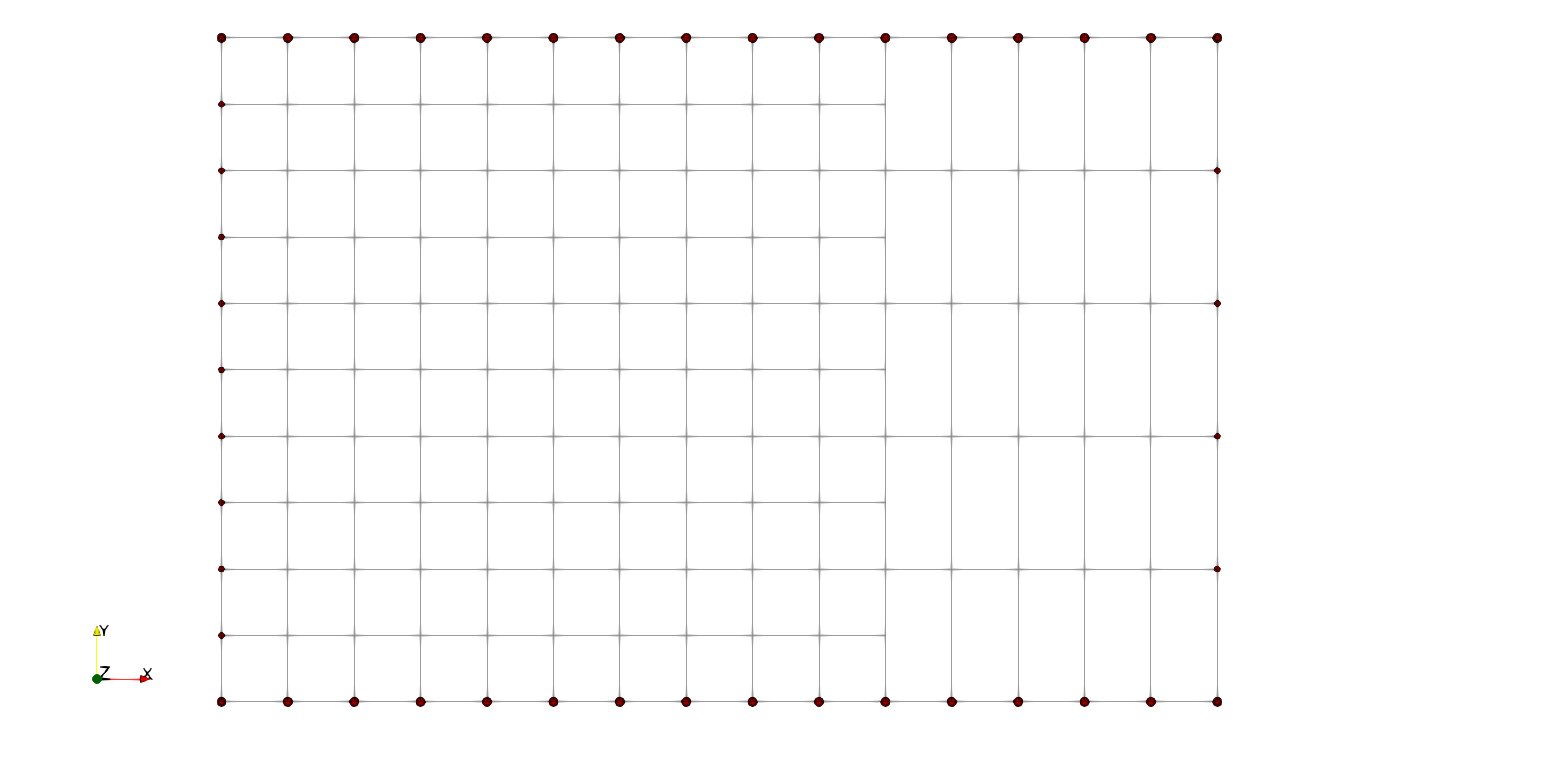
\includegraphics[width=0.9\linewidth]{figuras/tutorial_malha_5.png}
	\caption{Malha gerada no tutorial 5}
	\label{fig:tutorial_malha5}
\end{figure}

\begin{verbatim}
	mp_mapper *mp = mp_create();
    sim_domain *sd = sd_create(mp);
    sd_add_higtree(sd, root1);
    sd_add_higtree(sd, root2);

    for(int i =0; i < 4; i++) {
        sd_add_boundary(sd, sb[i]); /*Adds all boundaries*/
    }
\end{verbatim}

Após tudo isso, criamos de fato o domínio, representado pela estrutura \texttt{sim\_domain}. Adicionamos então as malhas e as condições de contorno ao domínio.

\begin{verbatim}
	it = higcit_create_all_leaves(root1);
    int size = mp_assign_from_celliterator(mp, it, 0);
    higcit_destroy(it);

    it = higcit_create_all_leaves(root2);
    size = mp_assign_from_celliterator(mp, it, size);
    higcit_destroy(it);
\end{verbatim}

Por fim, fazemos o assignment para o \textit{mapper} das células do domínio. a variável size guarda a quantidade de células no domínio. Isso será importante para o próximo tutorial.

%%%%%%%%%%%%%%%%%%%%%%%%%%%%%%%%%%%%%%%%%%%%%%%%%%%%%%%%%%%%%%%%%%%%%%%%%%%%%%%%%%%%%%%%%%
%%%%%%%%%%%%%%%%%%%%%%%%%%%%%%%%%%%%%%%%%%%%%%%%%%%%%%%%%%%%%%%%%%%%%%%%%%%%%%%%%%%%%%%%%%

\section{Tutorial 6 - Poisson 2D}
\label{sec:tut6}

Usando o domínio criado no tutorial anterior, resolvemos a equação de Poisson
\[
	\nabla^2u(x,y) = g(x,y), (x,y) \in \Omega
\]
Com condições de contorno
\[
	u(x,y) = f(x,y), (x,y) \in \partial \Omega
\]
Para a discretização do laplaciano, será empregada a discretização por diferenças finitas centradas:
\[
	\frac{U_{i+1,j}-2U_{i,j}+U_{i-1,j}}{\Delta x^2} + \frac{U_{i,j+1}-2U_{i,j}+U_{i,j-1}}{\Delta y^2} = g(x_i, y_j)
\]
Usaremos o método da solução manufaturada para verificar erros, dessa forma, tomaremos $f$ como uma restrição da solução analítica $u$ para a fronteira.

Duas estruturas serão essenciais na resolução desse problema: o \textit{stencil} e o \textit{solver}. O \textit{stencil} é a estrutura que guarda o peso de cada vizinho relacionado a uma célula específica, pesos esses usados para definir o sistema linear a ser resolvido. O \textit{solver} é responsável por montar o sistema linear e resolvê-lo.

\begin{verbatim}
	#include "solver.h"
\end{verbatim}

Precisamos apenas acrescentar essa biblioteca. o \textit{stencil} está implementado em \texttt{domain.h}.

\begin{verbatim}
	real u(real x, real y);
	real g(real x, real y);
\end{verbatim}

Essas funções são como descritas acima. No arquivo do tutorial, há uma série de casos para esse problema.

\begin{verbatim}
	sim_stencil *stn = stn_create();
	solver *slv = slv_create(SOLVER_ANY, 0, size);
	sd_set_interpolator_order(sd, 3);
    slv_set_maxnonzeros(slv, 300); 
\end{verbatim}

Criamos o \textit{solver} e o \textit{stencil}. O solver possui implementações com diversas engines. A engine padrão utiliza a biblioteca PETSc. Definimos aqui a ordem do polinônio interpolador para $3$ (\ref{sec:poly}). Por fim, definimos a quantidade máxima de entradas não nulas por linha na matriz do sistema. Para cada ponto não central do stencil, usa-se no máximo $60$ pontos para interpolação. Como usamos $4$ pontos não centrais, $300$ entradas não nulas são suficientes.

\begin{verbatim}
	for(it = sd_get_domain_celliterator(sd); 
	!higcit_isfinished(it); higcit_nextcell(it)) {
        hig_cell *c = higcit_getcell(it);
        Point ccenter;
        Point cdelta;
        hig_get_center(c, ccenter);
        real cx = ccenter[0];
        real cy = ccenter[1];
        hig_get_delta(c, cdelta);
        real dx = cdelta[0];
        real dy = cdelta[1];
        dy *= 1.0;

        /* Defines the points for a 5-point stencil*/
        Point center = {cx     , cy     };
        Point left   = {cx - dx, cy     };
        Point right  = {cx + dx, cy     };
        Point top    = {cx,      cy + dy};
        Point bottom = {cx,      cy - dy};

        stn_reset(stn);
        stn_set_rhs(stn, g(cx, cy));  // right side
        
        sd_get_stencil(sd, center, center, 
		(-2.0/(dx*dx)-2.0/(dy*dy)), stn);
        sd_get_stencil(sd, center, left,    (1.0/(dx*dx)), stn);
        sd_get_stencil(sd, center, right,   (1.0/(dx*dx)), stn);
        sd_get_stencil(sd, center, top,     (1.0/(dy*dy)), stn);
        sd_get_stencil(sd, center, bottom,  (1.0/(dy*dy)), stn); 

        int *ids = stn_get_ids(stn);
        real *vals = stn_get_vals(stn);
        int numelems = stn_get_numelems(stn);

        int cgid = mp_lookup(mp, hig_get_cid(c));
        slv_set_Ai(slv, cgid, numelems, ids, vals);
        slv_set_bi(slv, cgid, stn_get_rhs(stn));
    }
	higcit_destroy(it);
\end{verbatim}

Iteramos em todas as folhas de todas as árvores do domínio (criamos o iterador usando \texttt{sd\_get\_}

\texttt{domain\_celliterator()}). Para cada ponto apontado pelo iterador, pegamos os vizinhos. Os pesos dos vizinhos são calculados usando a função \texttt{sd\_get\_stencil()}. Então extraímos esses pesos usando \texttt{stn\_get\_ids()} e \texttt{stn\_get\_values()}. Esses valores são colocados na linha pertencente ao ponto central usando \texttt{slv\_set\_Ai()}. Note que o stencil também calcula o lado direito do sistema,se adaptando as condições de contorno, o que possibilita-nos definir o rhs usando \texttt{slv\_set\_bi()}. Para cada iteração, resetamos o stencil.
\begin{verbatim}
	slv_assemble(slv);
	slv_solve(slv);
\end{verbatim}

Usamos essas funções para montar o sistema definitivamente e resolvê-lo. Podemos então acessar os resultados calculados usando \texttt{slv\_get\_xi()} ou \texttt{slv\_get\_x()}.

%%%%%%%%%%%%%%%%%%%%%%%%%%%%%%%%%%%%%%%%%%%%%%%%%%%%%%%%%%%%%%%%%%%%%%%%%%%%%%%%%%%%%%%%%%%
%%%%%%%%%%%%%%%%%%%%%%%%%%%%%%%%%%%%%%%%%%%%%%%%%%%%%%%%%%%%%%%%%%%%%%%%%%%%%%%%%%%%%%%%%%%

\section{Tutorial 7 - Equação de Helmholtz vetorial nas faces}
\label{sec:tut7}

Neste tutorial, resolvemos uma equação de Helmholtz vetorial nas faces do domínio. O problema pode ser escrito através de duas equações desacopladas:
$$ -\nabla^2u(x,y) + k^2u(x,y) = f_1(x,y) $$
$$ -\nabla^2v(x,y) + k^2v(x,y) = f_2(x,y) $$
A variável $u$ representa a solução ao longo do eixo $x$ e é armazenada nas faces de dimensão 0, enquanto a variável $v$ é a solução no eixo $y$, armazenada nas faces de dimensão 1. O código adotado encontra-se no arquivo \textit{tutorial07-2d.c}.

Como estamos lidando com variáveis nas faces, precisamos criar domínios de faces (\texttt{sim\_facet\_domain}). O trecho a seguir ilustra a criação de dois domínios (um para cada eixo):
\begin{verbatim}
    sim_facet_domain *sfd[2];
    for(int dim = 0; dim < 2; dim++) {
        sfd[dim] = sfd_create(NULL, dim);
        sfd_add_higtree(sfd[dim], root);
        set_dirichlet_boundary_conditions(sfd[dim]->cdom, lo, hi, 
                                          nc, dim == 0? u : v);
        sfd_set_interpolator_order(sfd[dim], 3);
        sfd_adjust_facet_ids(sfd[dim]); 
\end{verbatim}
A função \texttt{sfd\_adjust\_facet\_ids()} é crucial aqui, pois lida com faces que possuem a mesma coordenada de centro, ajustando seus identificadores.

Em seguida, o código atribui identificadores globais iterando pelas faces de interesse.
\begin{verbatim}
        int dim_of_interest[2] = {1-dim, dim}; 
        higcit_celliterator *cit = higcit_create_all_leaves(
                                   sfd_get_higtree(sfd[dim],0));
        higfit_facetiterator *fit = higfit_create_allfacets(cit, 
                                    dim_of_interest); 
                                    
        size = mp_assign_from_facetiterator(
               sfd_get_domain_mapper(sfd[dim]), fit, start);
        start = size;
        higfit_destroy(fit);
    }
\end{verbatim}
O vetor \texttt{dim\_of\_interest} define qual dimensão estamos iterando.Atribuirmos os IDs de $u$ primeiro e os de $v$ em seguida (através da variável \texttt{start}). Isso possibilita montarmos apenas um sistema linear para resolução. Isso não é vantajoso nesse caso, mas é necessário no caso em que as variáveis são acopladas. 

A matriz é montada e resolvida de forma análoga ao exemplo anterior.

%%%%%%%%%%%%%%%%%%%%%%%%%%%%%%%%%%%%%%%%%%%%%%%%%%%%%%%%%%%%%%%%%%%%%%%%%%%%%%%%%%%%%%%%%%%
%%%%%%%%%%%%%%%%%%%%%%%%%%%%%%%%%%%%%%%%%%%%%%%%%%%%%%%%%%%%%%%%%%%%%%%%%%%%%%%%%%%%%%%%%%%

\section{Tutorial 8 - Poisson paralelo 2D}
\label{sec:tut8}

Nesta seção, avançamos para a resolução de equações diferenciais em paralelo, particionando o domínio entre múltiplos processadores com o uso da biblioteca MPI. O código base está no arquivo \textit{tutorial08-2d.c}. 

Primeiramente, inicializamos as variáveis do MPI para resgatar o identificador local (\texttt{myrank}) e o número total de processos (\texttt{ntasks}):
\begin{verbatim}
    MPI_Comm_rank(MPI_COMM_WORLD, &myrank);
    MPI_Comm_size(MPI_COMM_WORLD, &ntasks);
\end{verbatim}

Para dividir as árvores que compõem a malha, introduzimos o grafo de partição (\texttt{partition\_graph}) e o balanceador de carga (\texttt{load\_balancer}):
\begin{verbatim}
    partition_graph *pg = pg_create(MPI_COMM_WORLD);
    
    sim_domain *sd = sd_create(NULL);
    sd_create_boundary(root, sd, DIRICHLET);
    set_dirichlet_boundary_conditions(sd);

    load_balancer *lb = lb_create(MPI_COMM_WORLD, 1);
    if (myrank == 0) {
        lb_add_input_tree(lb, root, true, 0);
    } else {
        hig_destroy(root);
    }
    lb_calc_partition(lb, pg);
\end{verbatim}
O \texttt{load\_balancer} é o responsável por efetivamente calcular a partição das HiG-Trees através da função \texttt{lb\_calc\_partition()}. Após isso, resgatamos a parcela do domínio que pertence ao processador atual e adicionamos ao domínio base \texttt{sd}.

O passo final e mais importante da paralelização é criar o domínio particionado e sincronizar os IDs globais através da rede:
\begin{verbatim}
    psd = psd_create(sd, pg);
    psd_synced_mapper(psd); 
    int localdomainsize = psd_get_local_domain_size(psd);
\end{verbatim}
A estrutura \texttt{psim\_domain} encapsula o domínio para uso paralelo. A chamada de \texttt{psd\_synced\_mapper()} faz automaticamente todo o trabalho pesado de sincronização de IDs no mapeador, o qual, caso contrário, precisaria ser feito manualmente. Com a matriz e o vetor local definidos, o \textit{solver} resolve o sistema linear distribuído e salva um arquivo \textit{.vtk} para o domínio de cada processador, facilitando a visualização dos resultados parciais.

%%%%%%%%%%%%%%%%%%%%%%%%%%%%%%%%%%%%%%%%%%%%%%%%%%%%%%%%%%%%%%%%%%%%%%%%%%%%%%%%%%%%%%%%%%%
%%%%%%%%%%%%%%%%%%%%%%%%%%%%%%%%%%%%%%%%%%%%%%%%%%%%%%%%%%%%%%%%%%%%%%%%%%%%%%%%%%%%%%%%%%%

\section{Tutorial 9 -- Equação de Advecção e Métodos Numéricos}
\label{sec:tut9}

Nesta etapa vamos explorar um problema dependente do tempo, resolvendo a equação de advecção linear:
$$ u_t + v_1u_x + v_2u_y = 0 $$
assumindo velocidades positivas $v_1, v_2 > 0$ e uma condição inicial $u(x,y,0) = f(x,y)$. Para lidar com a evolução temporal, utilizamos a estrutura \texttt{distributed\_property} (propriedade distribuída), que armazena os valores da simulação em um dado instante e permite consultar esses valores passados para calcular o próximo passo de tempo.
\begin{verbatim}
    distributed_property *dpu_last = psd_create_property(psd);
    distributed_property *dpu_now = psd_create_property(psd);
\end{verbatim}
Veremos dois métodos distintos para lidar com as derivadas espaciais desta equação.

\subsection{Método de Lax-Friedrichs}
O primeiro método se encontra no arquivo \textit{tutorial09-lax-2d.c}. O esquema numérico de Lax-Friedrichs estabiliza a solução substituindo o termo $u_{i,j}$ (centro) pela média de seus quatro vizinhos ortogonais e aproximando a derivada espacial por diferenças centrais. O núcleo da iteração no tempo se dá pela linha:
\begin{verbatim}
    real next_u = (uright+uleft+utop+ubottom)/4 
                  - ((v1*dt)/(2*dx))*(uright-uleft) 
                  - ((v2*dt)/(2*dy))*(utop-ubottom);
                  
    dp_set_value(dpu_now, cgid, next_u);
\end{verbatim}
Este método explícito requer que o valor de $dt$ respeite as condições numéricas de estabilidade (CFL), que são calculadas previamente baseadas no menor delta da malha e nas velocidades $v_1, v_2$.

\subsection{Método Upwind}
O segundo método (\textit{tutorial09-upwind-2d.c}) aproveita a direção do escoamento da física do problema. Sabendo que $v_1 > 0$ e $v_2 > 0$, a informação se propaga da esquerda para a direita, e de baixo para cima. O método \textit{Upwind} (contra o fluxo) usa então as diferenças atrasadas (backward) para calcular as derivadas espaciais, dependendo apenas do centro, da vizinhança à esquerda e da vizinhança abaixo:
\begin{verbatim}
    real uleft = sd_dp_interpolate(localdomain, dpu_last, 
                                   ccenter, left, stn);
    real ubottom = sd_dp_interpolate(localdomain, dpu_last, 
                                     ccenter, bottom, stn);
    real ucenter = dp_get_value(dpu_last, cgid);

    real next_u = ucenter - ((v1*dt)/dx)*(ucenter-uleft) 
                  - ((v2*dt)/dy)*(ucenter-ubottom);
\end{verbatim}
Neste contexto, vale notar que, devido à simplicidade da aproximação em primeira ordem espacial, o erro numérico acumula. A própria documentação do código sugere utilizar interpoladores de ordem 1 para a propriedade, indicando que esse método é mais recomendável para simulações executadas sobre malhas regulares. Ao fim do laço, assim como em Lax-Friedrichs, os valores são atualizados transferindo os dados de \texttt{dpu\_now} para \texttt{dpu\_last}.
%%%%%%%%%%%%%%%%%%%%%%%%%%%%%%%%%%%%%%%%%%%%%%%%%%%%%%%%%%%%%%%%%%%%%%%%%%%%%%%%%%%%%%%%%%
%%%%%%%%%%%%%%%%%%%%%%%%%%%%%%%%%%%%%%%%%%%%%%%%%%%%%%%%%%%%%%%%%%%%%%%%%%%%%%%%%%%%%%%%%%

\section{Parte I}

{Introdução}

Problemas que necessitam de malhas com boa resolução para capturar fenômenos físicos.

\begin{figure}[H]
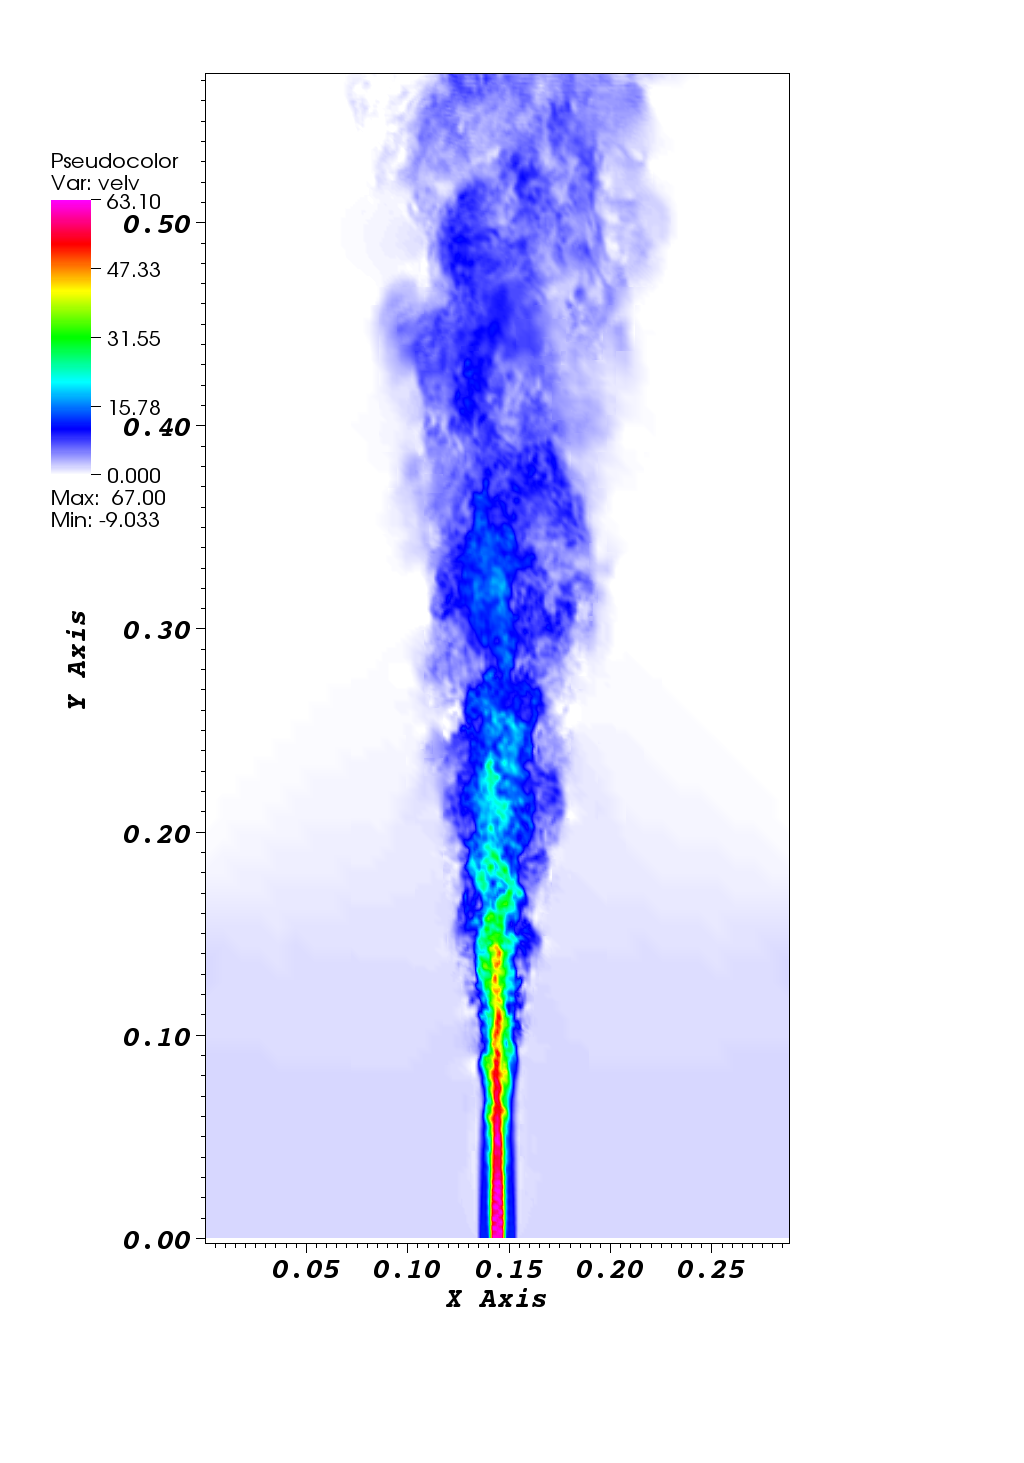
\includegraphics[width=2in]{figuras/wccmjet.png}
\end{figure}

\begin{figure}[H]
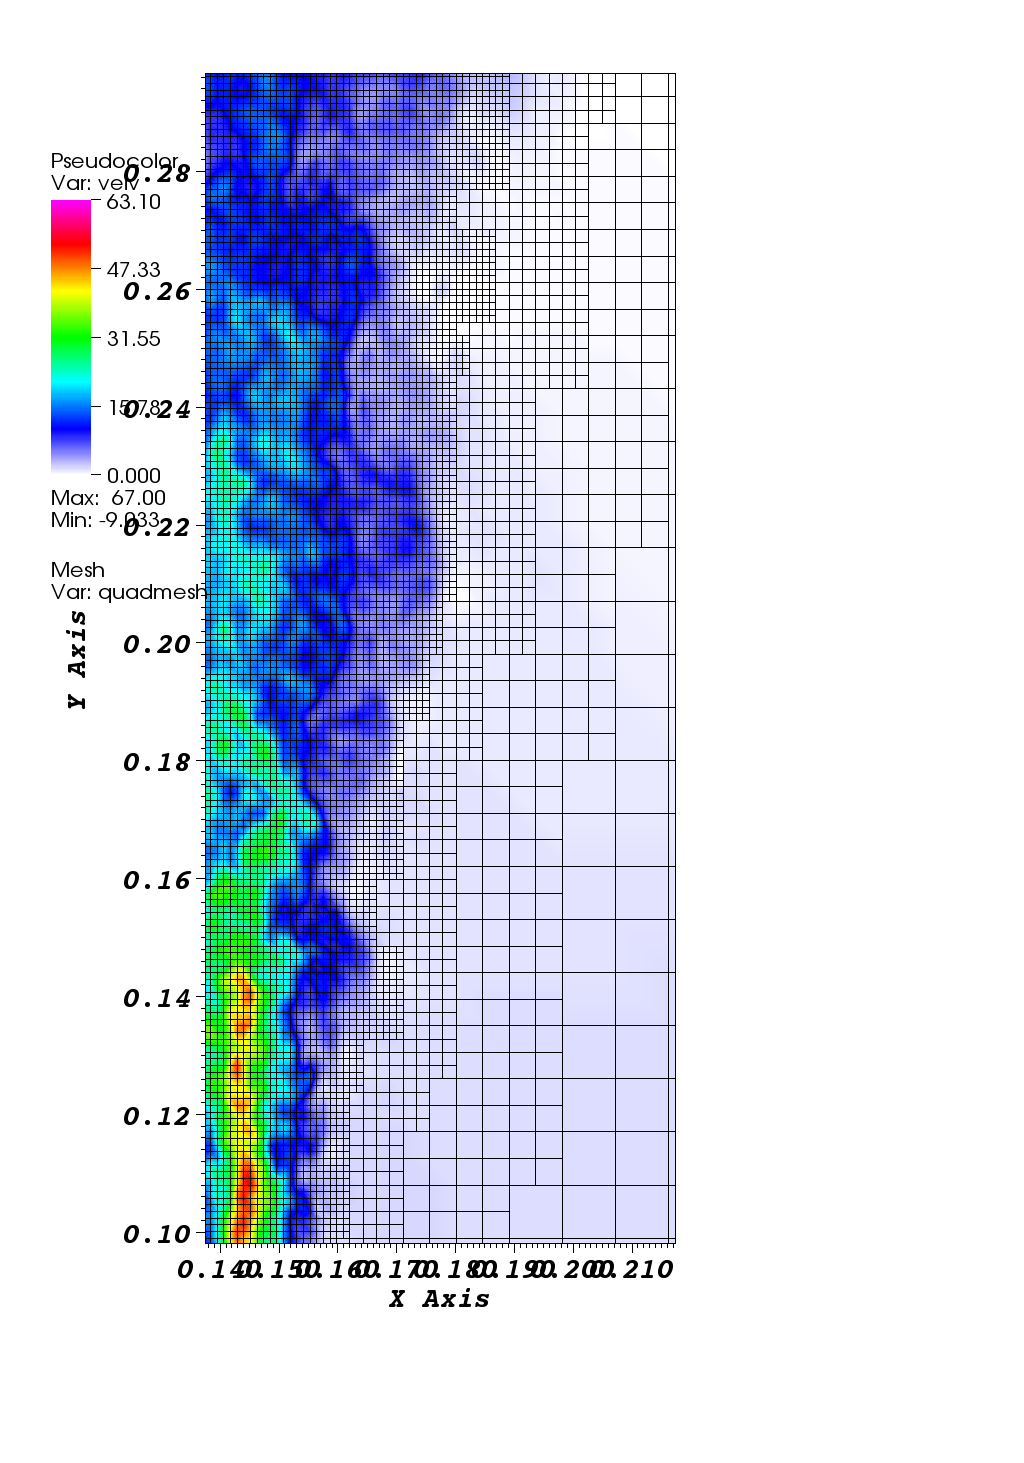
\includegraphics[width=2in]{figuras/wccmjetz.png}
\end{figure}


%%%%%%%%%%%%%%%%%%%%%%%%%%%%%%%%%%%%%%%%%%%%%%%%%%%%%%%%%%%%%%%%%%%%%%%

\bf{Definição:}

$G_{l,m}$: $m$-ésimo bloco de um nível de refinamento $l$ ({\it patch}).

\vspace{1pc}
{Para cada dois blocos $G_{l, i}$ e $G_{l, j}$, tem-se que $G_{l,i} \cap G_{l,j} = \emptyset$. Assim, a malha do nível $l$ por $\displaystyle{G_l = \bigcup_{k=1}^{n_l}G_{l,k}}$ e a malha bloco-estruturada é dada por $\displaystyle{G = \bigcup_{l} G_l}$.}

\vspace{1pc}
{Propriedade:}
Blocos em níveis diferentes consecutivos precisam estar propriamente ani\-nhados, ou seja,
\begin{enumerate}
\item um bloco no nível fino deve começar e terminar no canto de uma célula do próximo nível mais grosso; e
\item para cada canto de um bloco do nível fino, existe pelo menos uma célula do próximo nível mais grosso em todas as direções que separa este bloco fino de uma célula do segundo próximo nível mais grosso (a menos se ele toca a fronteira do domínio físico).
\end{enumerate}


%%%%%%%%%%%%%%%%%%%%%%%%%%%%%%%%%%%%%%%%%%%%%%%%%%%%%%%%%%%%%%%%%%%%%%%

\bf{Refinamento adaptativo de malhas (AMR)}

Berger e Colella (1989), Berger e Oliger (1984) e Berger e Rigoutsos (1991).

\vspace{0.5pc}

\begin{itemize}

\item Refinamento adaptativo em regiões de interesse.
\vspace{1pc}

\item Tempo computacional.
\vspace{1pc}

\item Malhas bloco-estruturadas (Diferenças finitas).
\vspace{1pc}

\end{itemize}


%%%%%%%%%%%%%%%%%%%%%%%%%%%%%%%%%%%%%%%%%%%%%%%%%%%%%%%%%%%%%%%%%%%%%%%%%%%%

\bf{Blocos não propriamente aninhados:}

\begin{figure}
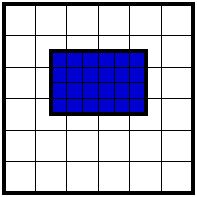
\includegraphics[width=1.8in]{figuras/alvaro_malha1.png}
\put(-105,120){{\tiny $G_{1,1}$}}
\put(-82,102){{\tiny $G_{2,1}$}}
\caption{Viola primeira propriedade.}
\end{figure}

\begin{figure}
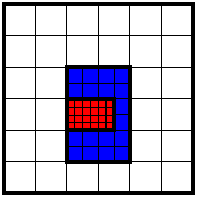
\includegraphics[width=1.8in]{figuras/alvaro_malha2.png}
\put(-105,120){{\tiny $G_{1,1}$}}
\put(-82,95){{\tiny $G_{2,1}$}}
\put(-105,55){{\tiny $G_{3,1}$}}
\caption{Viola segunda propriedade.}
\end{figure}

%%%%%%%%%%%%%%%%%%%%%%%%%%%%%%%%%%%%%%%%%%%%%%%%%%%%%%%%%%%%%%%%%%%

\bf{Discretização espacial}

Malha deslocada, diferenças finitas e células fantasmas.
\begin{figure}
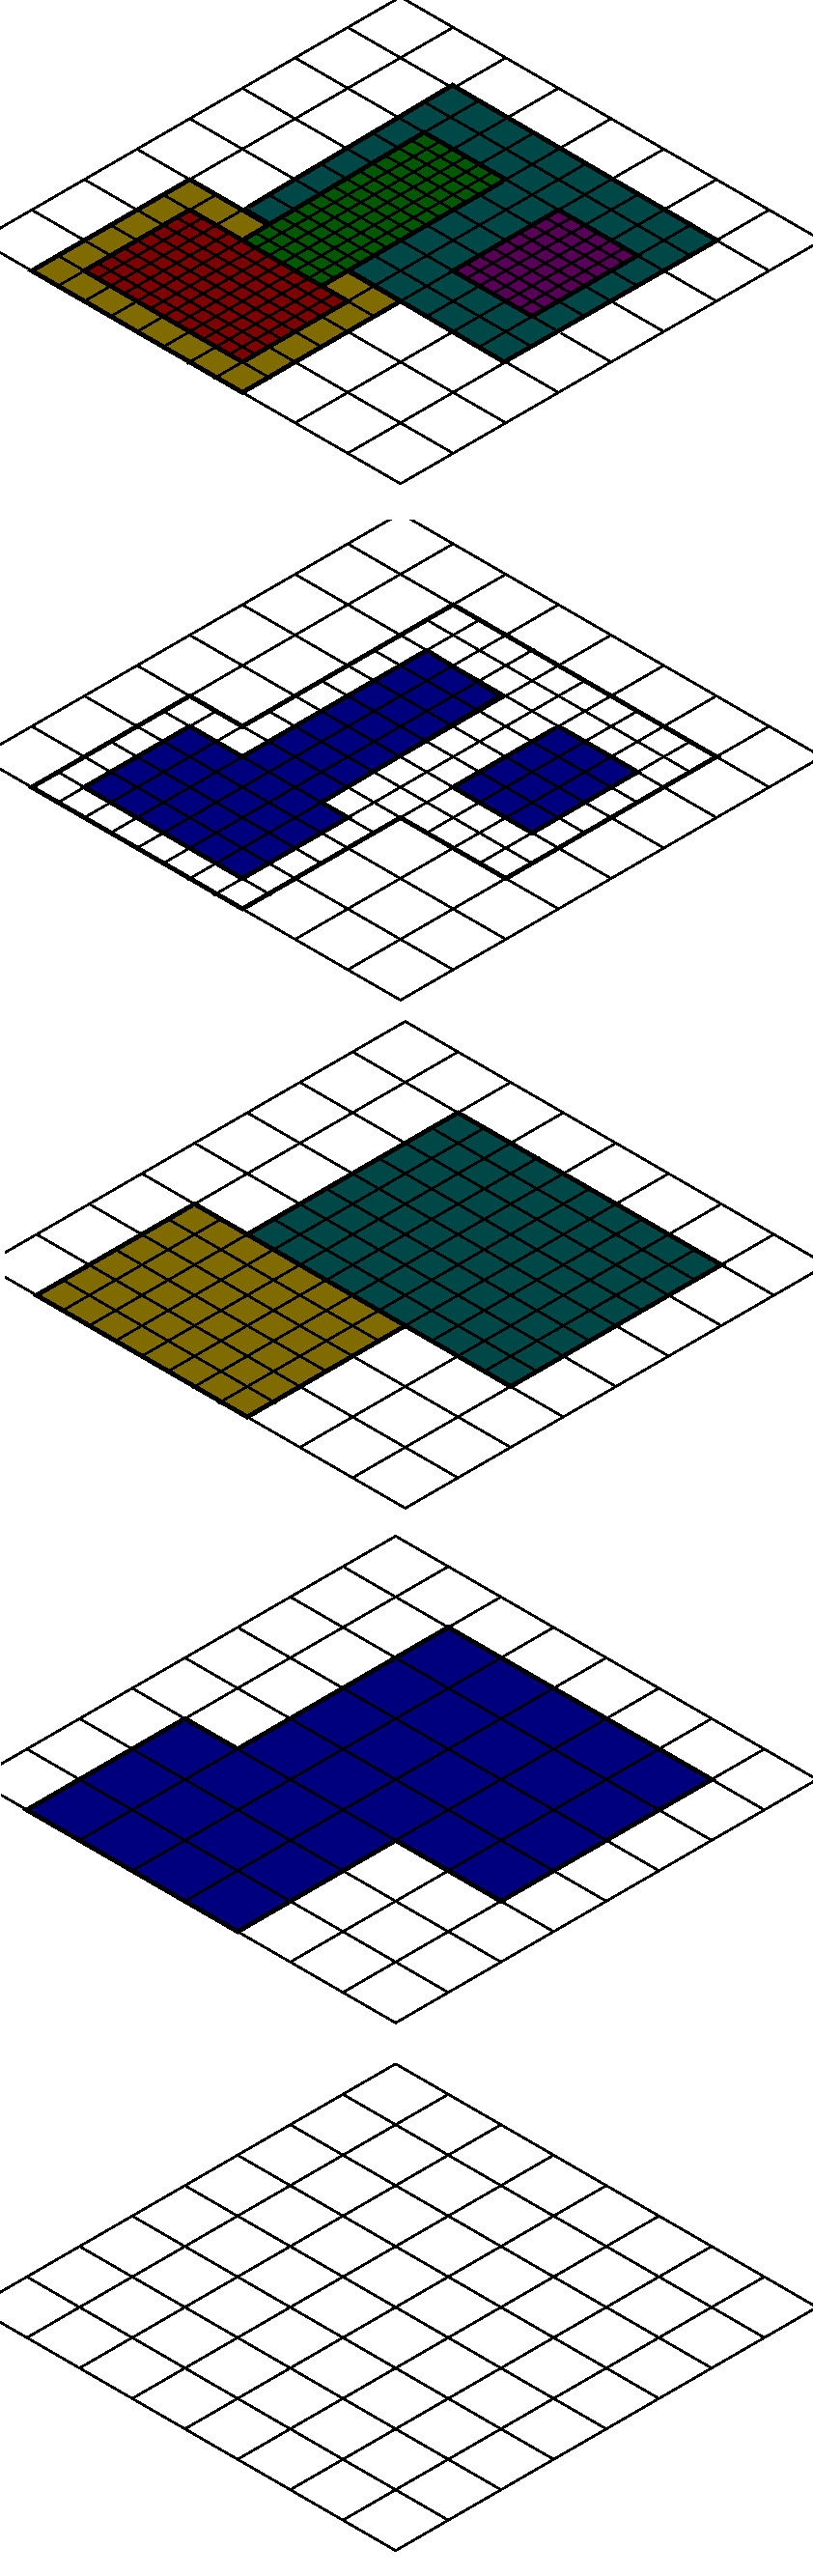
\includegraphics[width=0.7in]{figuras/all_mesh.png}
\caption{Malha bloco-estruturada.}
\end{figure}

\begin{figure}
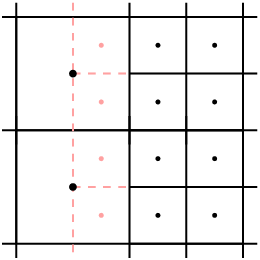
\includegraphics[width=1.6in]{figuras/ghosts.png}
\caption{Malha 2D com células fantasmas.}
\end{figure}


%%%%%%%%%%%%%%%%%%%%%%%%%%%%%%%%%%%%%%%%%%%%%%%%%%%%%%%%%%%%%%%%%%%%%%%%%%


{\footnotesize Componente da velocidade na direção do escoamento em um plano de corte central.}

%-------------------------------------------------------------------------------

%slide19

\bf{Escoamento turbulento}


{\footnotesize Corte transversal.}

%%%%%%%%%%%%%%%%%%%%%%%%%%%%%%%%%%%%%%%%%%%%%%%%%%%%%%%%%%%%%%%%%%%%%%%%%%%%%%%%%%%%%%%%%%%%%%%%%%%%%%%%%%%
% M-tree

\bf{Exemplos de malhas com a estrutura m-tree}
\begin{figure}
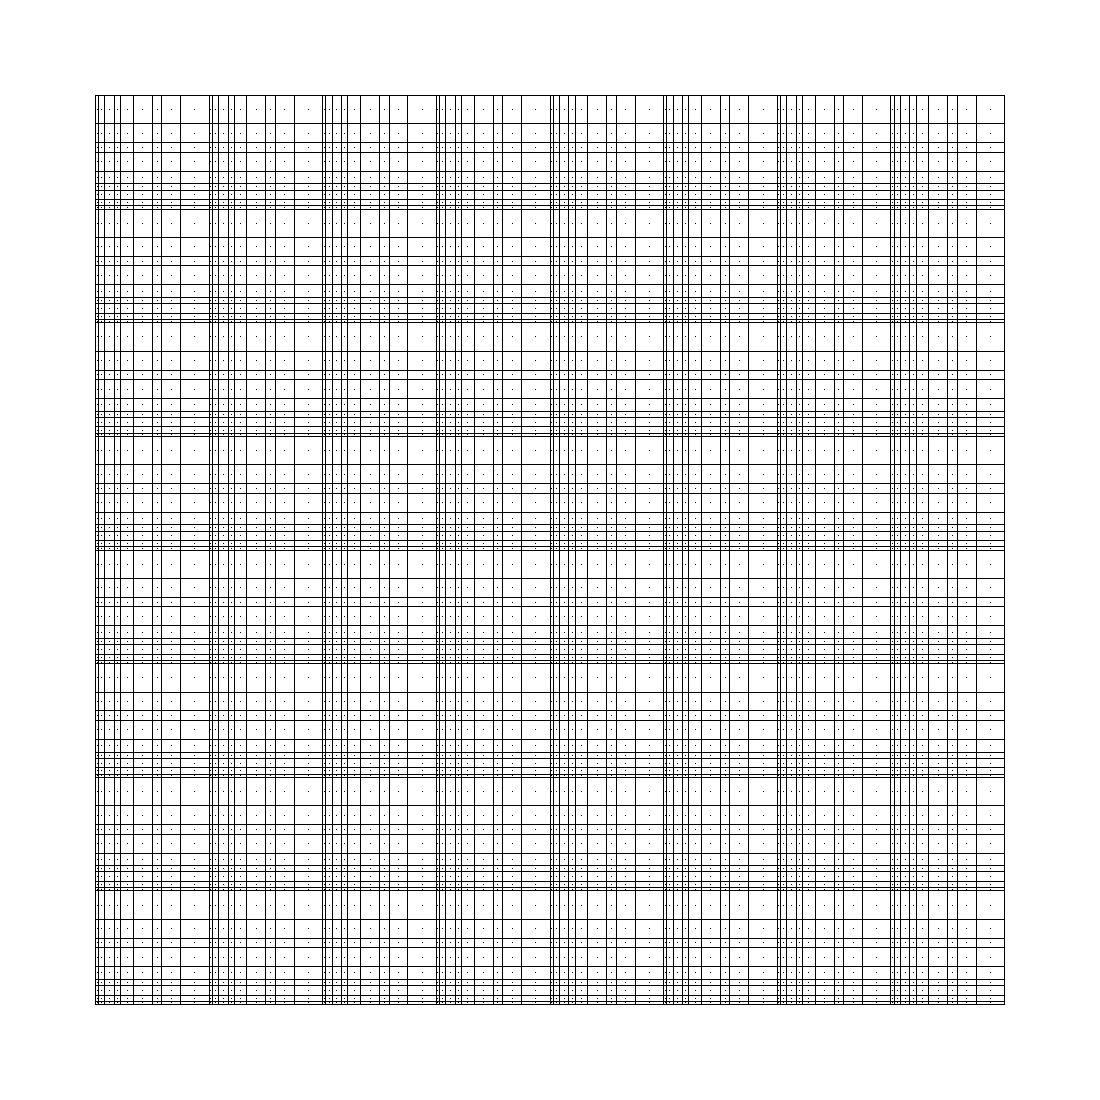
\includegraphics[width=2.5in]{figuras/fig1.png}
\caption{Malha com estrutura m-tree.}
\end{figure}

\begin{figure}
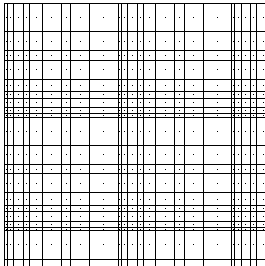
\includegraphics[width=2.1in]{figuras/mesh1zoom.png}
%\vspace{1pc}
\caption{Zoom da malha m-tree.}
\end{figure}


%%%%%%%%%%%%%%%%%%%%%%%%%%%%%%%%%%%%%%%%%%%%%%%%%%%%%%%%%%%%%%%%%%%%%%%%%%%%%%%%%%%%%%%%%%%%%%%%%%%%

\bf{Exemplos de malhas com a estrutura m-tree}
\begin{figure}
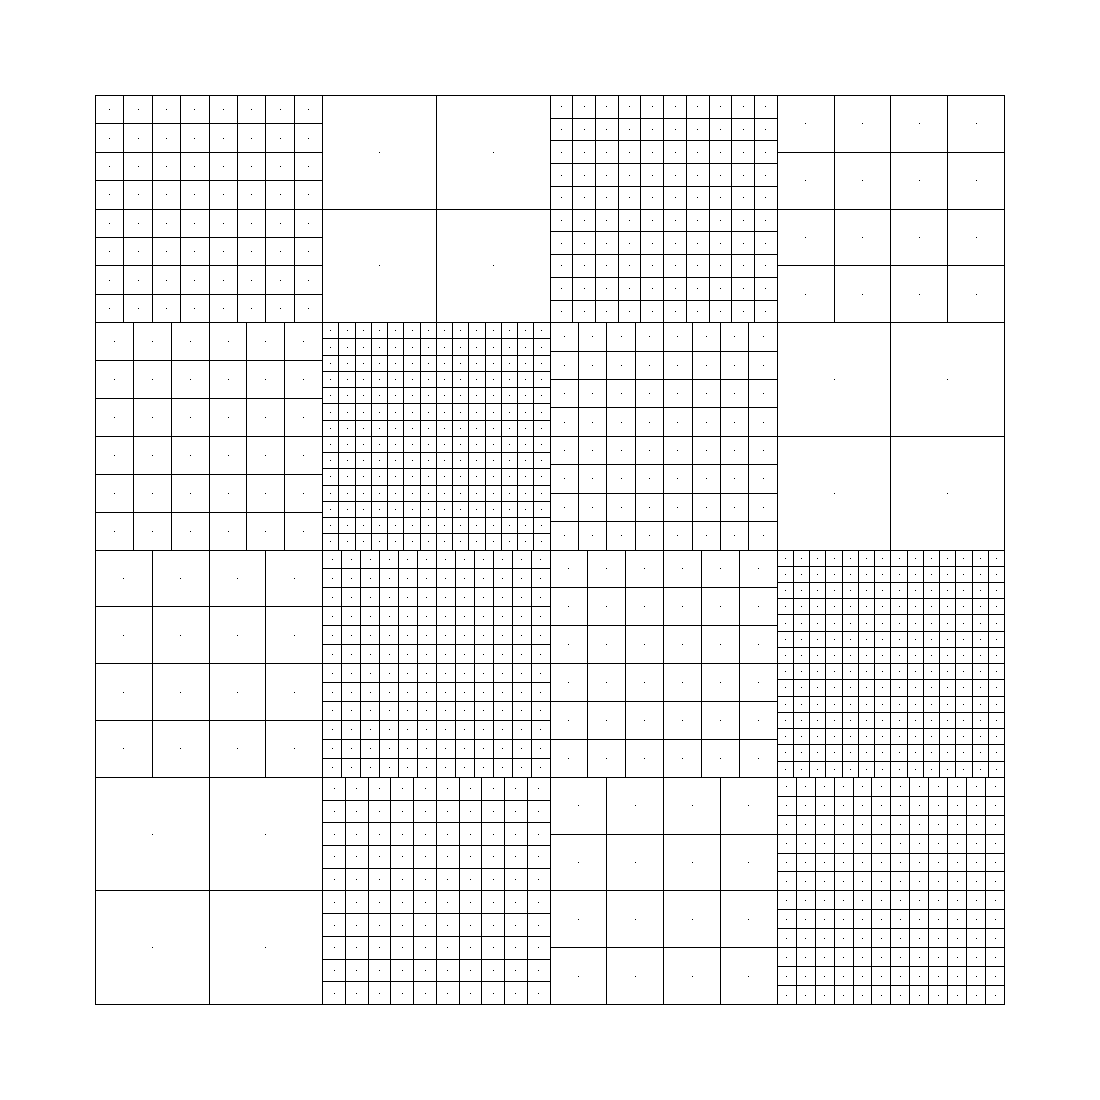
\includegraphics[width=2.5in]{figuras/fig2.png}
\caption{Malha com estrutura m-tree.}
\end{figure}

\begin{figure}
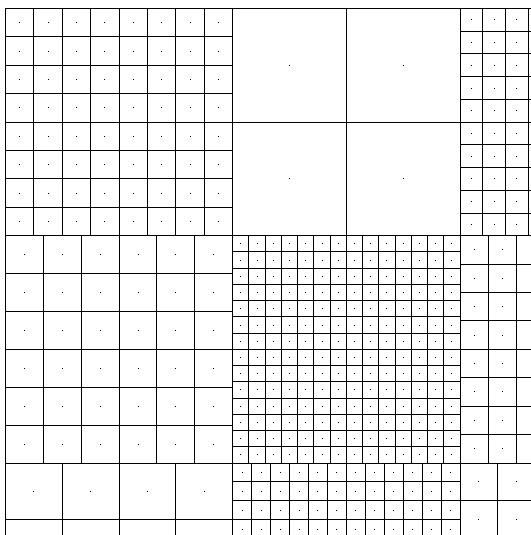
\includegraphics[width=2.1in]{figuras/mesh2zoom.png}
\caption{Zoom da malha m-tree.}
\end{figure}


%%%%%%%%%%%%%%%%%%%%%%%%%%%%%%%%%%%%%%%%%%%%%%%%%%%%%%%%%%%%%%%%%%%%%%%%%%%%%%%%%%%%%%%%%%%%%%%%%%%%

\bf{Exemplos de malhas com a estrutura m-tree}

\begin{figure}
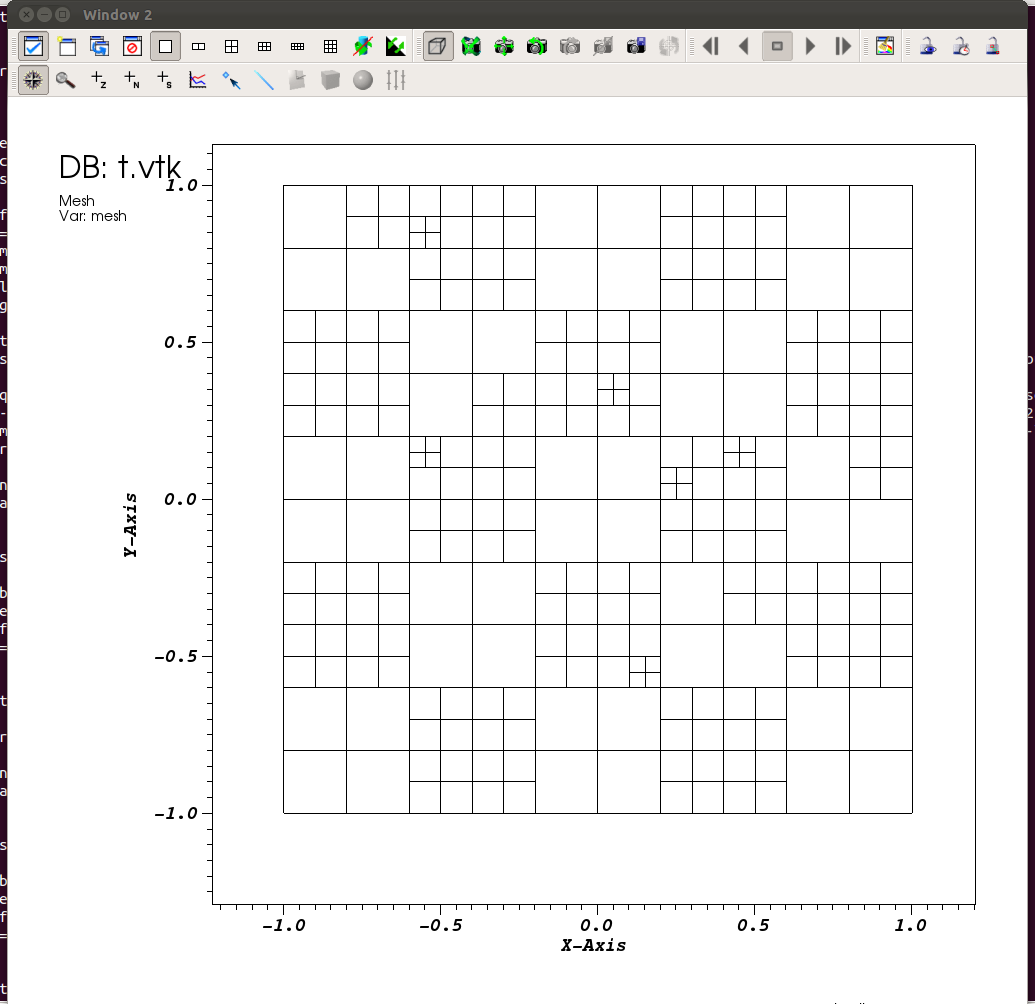
\includegraphics[width=2.8in]{figuras/level-0.png}
%\caption{Malha 2D com células fantasmas.}
\end{figure}

%%%%%%%%%%%%%%%%%%%%%%%%%%%%%%%%%%%%%%%%%%%%%%%%%%%%%%%%%%%%%%%%%%%%%%%%%%%%%%%%%%%%%%%%%%%%%%%%%%%%%%

\bf{Exemplos de malhas com a estrutura m-tree}

\begin{figure}
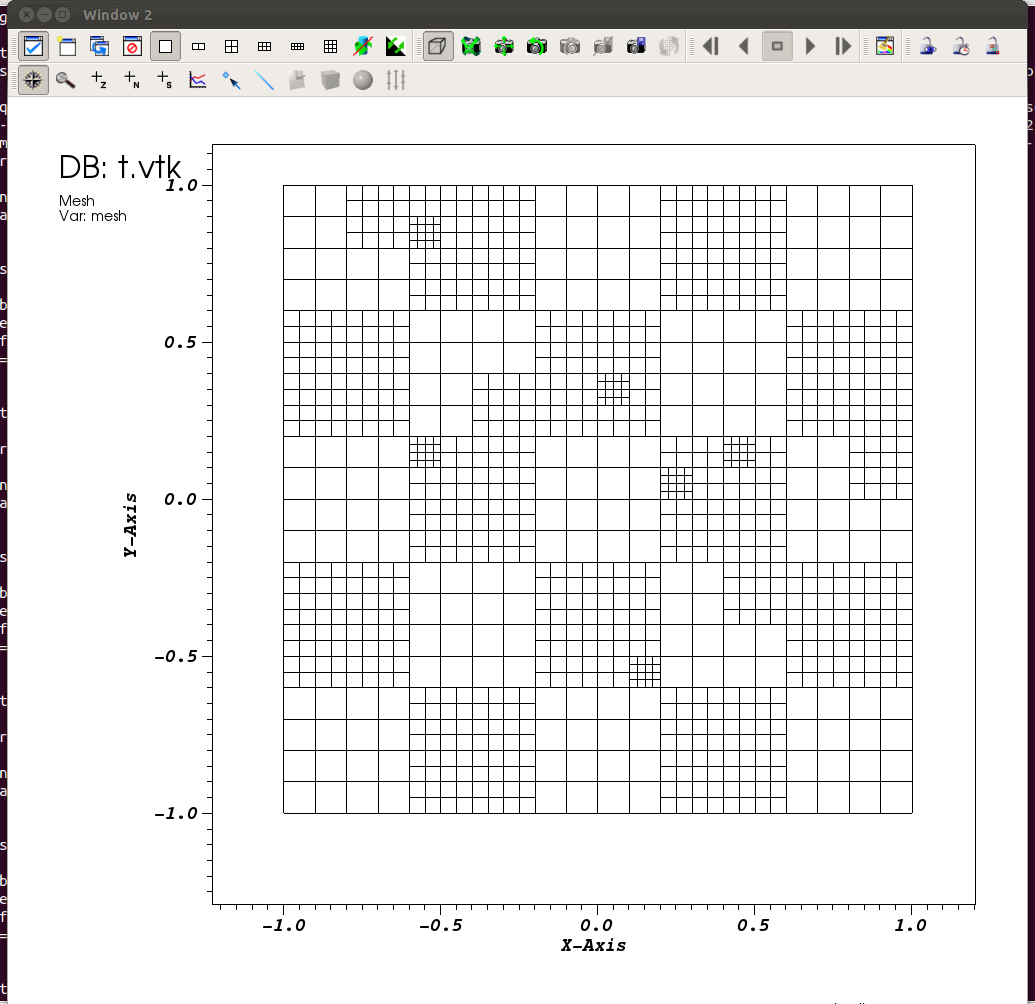
\includegraphics[width=2.8in]{figuras/level-1.png}
\end{figure}


%%%%%%%%%%%%%%%%%%%%%%%%%%%%%%%%%%%%%%%%%%%%%%%%%%%%%%%%%%%%%%%%%%%%%%%%%%%%%%%%%%

\bf{Exemplos de malhas com a estrutura m-tree}

\begin{figure}
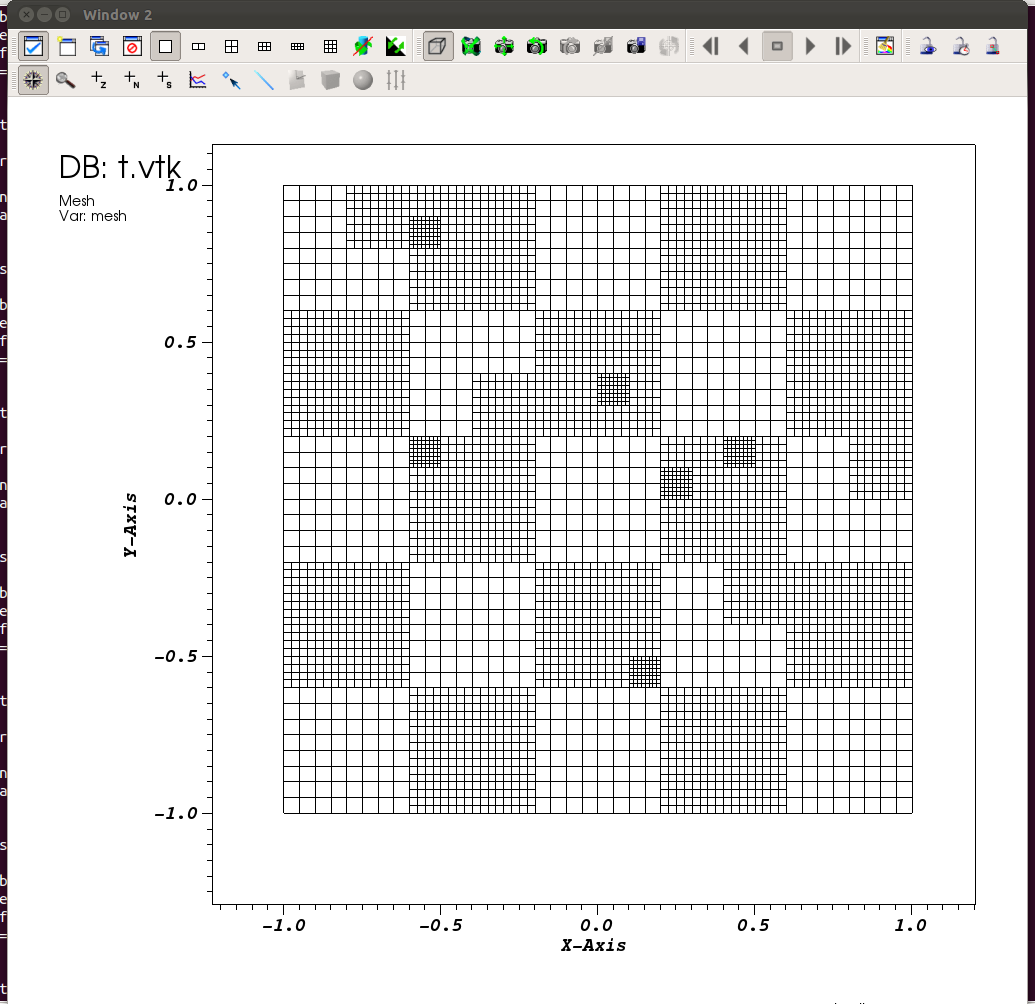
\includegraphics[width=2.8in]{figuras/level-2.png}
\end{figure}


%%%%%%%%%%%%%%%%%%%%%%%%%%%%%%%%%%%%%%%%%%%%%%%%%%%%%%%%%%%%%%%%%%%%%%%%%%%%%%%%

%%%%%%%%%%%%%%%%%%%%%%%%%%%%%%%%%%%%%%%%%%%%%%%%%%%%%%%%%%%%%%%%%%%%%%%%%%%%%%

\bf{Código m-tree 1.1}

Nessa versão, foram incluídas as seguintes funcionalidades:
\begin{enumerate}
\item Criação de malha com refinamento uniforme (cada célula pode ser
dividida em sub-células igualmente espaçadas, uma célula é independente das
demais).
\item Leitura de malha no formato AMR2D.
\item Escrita de malha no formato VTK2D.
\item Iteradores para:
\begin{enumerate}
\item percorrer todas as células da malha;
\item percorrer todas as células que intersectam um {\it bounding box};
\item percorrer todas as células vizinhas de uma célula;
\end{enumerate}
\item Operações para encontrar a célula que contém uma determinada
coordenada (ponto).
\end{enumerate}


%%%%%%%%%%%%%%%%%%%%%%%%%%%%%%%%%%%%%%%%%%%%%%%%%%%%%%%%%%%%%%%%%%%%%%%%%
\bf{Código m-tree 1.1}

Todos essas funcionalidades foram testadas. Os testes estão incluídos
no diretório atf-tests.

Deve-se instalar o ATF,
http://kyua.googlecode.com/files/atf-0.15.tar.gz .

Para instalar faça: ./configure; make; sudo make install.

Para rodar os 33 casos de teste criados, execute 'make test'.

Para avaliar a cobertura do código, execute 'make gcov'
(o resultado deve indicar $100\%$ de código
coberto).

%%%%%%%%%%%%%%%%%%%%%%%%%%%%%%%%%%%%%%%%%%%%%%%%%%%%%%%%%%%%%%%%%%%%%%%%%%

\bf{Malhas com estrutura m-tree: atividade da semana I}

{\bf Exercício:}

\begin{enumerate}
\item ``Varrer as folhas" (que são as células visíveis) de uma malha típica AMR *carregada para dentro do código da malha m-tree*.

\item Calcular uma função no centro de cada célula computacional e visualizar o gráfico em 2D.

\end{enumerate}

%-----------------------------------------------------------------------------

\bf{Formato do arquivo AMR para ser lido no m-tree }

\begin{enumerate}
 \item Domínio A1 B1 A2 B2 A3 B3
 \item Número de níveis
 \item Informação do nível: Espaçamento dx, dy e dz; quantidade de patches
 \item Informação do patch:
   \begin{itemize}
    \item Índices na correspondente malha uniforme, da primeira célula do patch (inferior esquerda): i, j e k
    \item Número de células em cada direção: nx, ny e nz
   \end{itemize}


\end{enumerate}


%%%%%%%%%%%%%%%%%%%%%%%%%%%%%%%%%%%%%%%%%%%%%%%%%%%%%%%%%%%%%%%%%%%%%%%%%%%%%%%%

\bf{Formato do arquivo AMR para ser lido no m-tree }

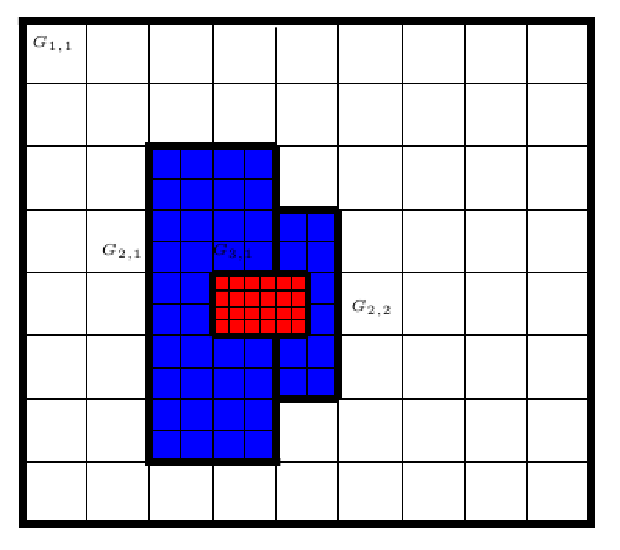
\includegraphics[height=5cm,width=5cm]{figuras/basicAMRmesh.pdf}
\textit{mesh1.amr}\\
0 0.9 0 0.8\\
3\\
0.1 0.1 1\\
1 1 9 8\\
0.05 0.05 2\\
5 3 4 10\\
9 5 2 6\\
0.025 0.025 1\\
13 13 6 4\\

No diretório exemplos encontram-se as funções utilizadas na atividade I.


%%%%%%%%%%%%%%%%%%%%%%%%%%%%%%%%%%%%%%%%%%%%%%%%%%%%%%%%%%%%%%%%%%%%%%%%

\section{Parte II}

\bf{Malhas com estrutura m-tree: atividade da semana II}

Vamos definir um vetor bidimensional para armazenar uma curva parametrizada (x(s),y(s)) - uma fronteira imersa. Vamos fazer um programa com um laço em s e, para cada ponto da curva, vamos localizar a folha em que ele se encontra e marcar uma vizinhança de ordem p. Vamos visualizar o resultado.

%%Aqui Atividades da segunda semana


\bf{Exemplo 1}
\textbf{Makefile}
\begin{verbatim}
initial : initial.c
	$(CC) $(OBJS) $(OPTS) -o initial initial.c $(LIBS)
\end{verbatim}
\textbf{Arquivo \textit{initial.c}}
\begin{verbatim}
#include<stdio.h>
#include<stdlib.h>
#include "higtree.h"
#include "higtree-io.h"

#if DIM ==2  // só compila para DIM=2
int main(int argc, char *argv[]) {
...
}
#endif
\end{verbatim}

\begin{verbatim}
Point l, h;  //point low and point high
\end{verbatim}
Três formas diferentes para assinar os valores dos pontos,\\
por exemplo $l(-1,-1)$ e $h(1,2)$.
\begin{itemize}
\item
\begin{verbatim}
for(int i = 0; i < DIM; i++){
  l[i] = -1
}
\end{verbatim}
\item
\begin{verbatim}
POINT_ASSIGN_SCALAR(l,-1.0)
\end{verbatim}
\item
\begin{verbatim}
h[0] = 1.0;
h[1] = 2.0;
\end{verbatim}
\end{itemize}
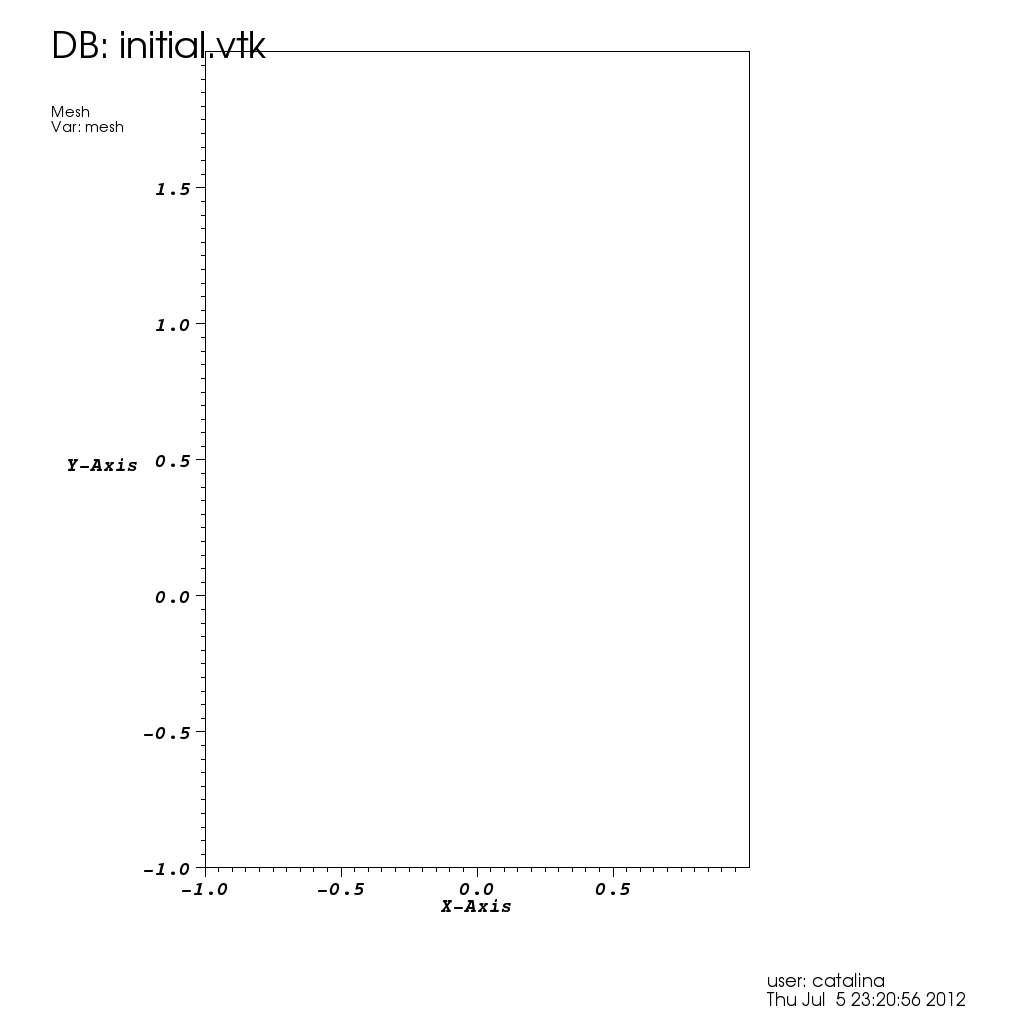
\includegraphics[height=3cm,width=3cm]{figuras/initial0000.png}
\vspace{0.4cm}
\textbf{Criar a Raiz}
\vspace{-0.3cm}
\begin{verbatim}
hig_cell *root = hig_create_root(l,h);
...
hig_destroy(root);
\end{verbatim}

\vspace{0.3cm}
\textbf{Visualizar a malha em arquivo VTK}
\begin{verbatim}
 FILE * fdout = fopen("initial.vtk", "w");
 if(fdout == NULL){
    // Mensagem de erro
    exit(1);
 }
 higio_print_in_vtk2d(fdout, root);
 fclose(fdout);
\end{verbatim}
\textbf{Subdividir o dominio principal}\\
Dividir em 4 na dir X e em 3 na dir Y.
\begin{verbatim}
 int num_cells[DIM];
 num_cells[0] = 4;
 num_cells[1] = 3;
 hig_refine_uniform(root,num_cells);
\end{verbatim}
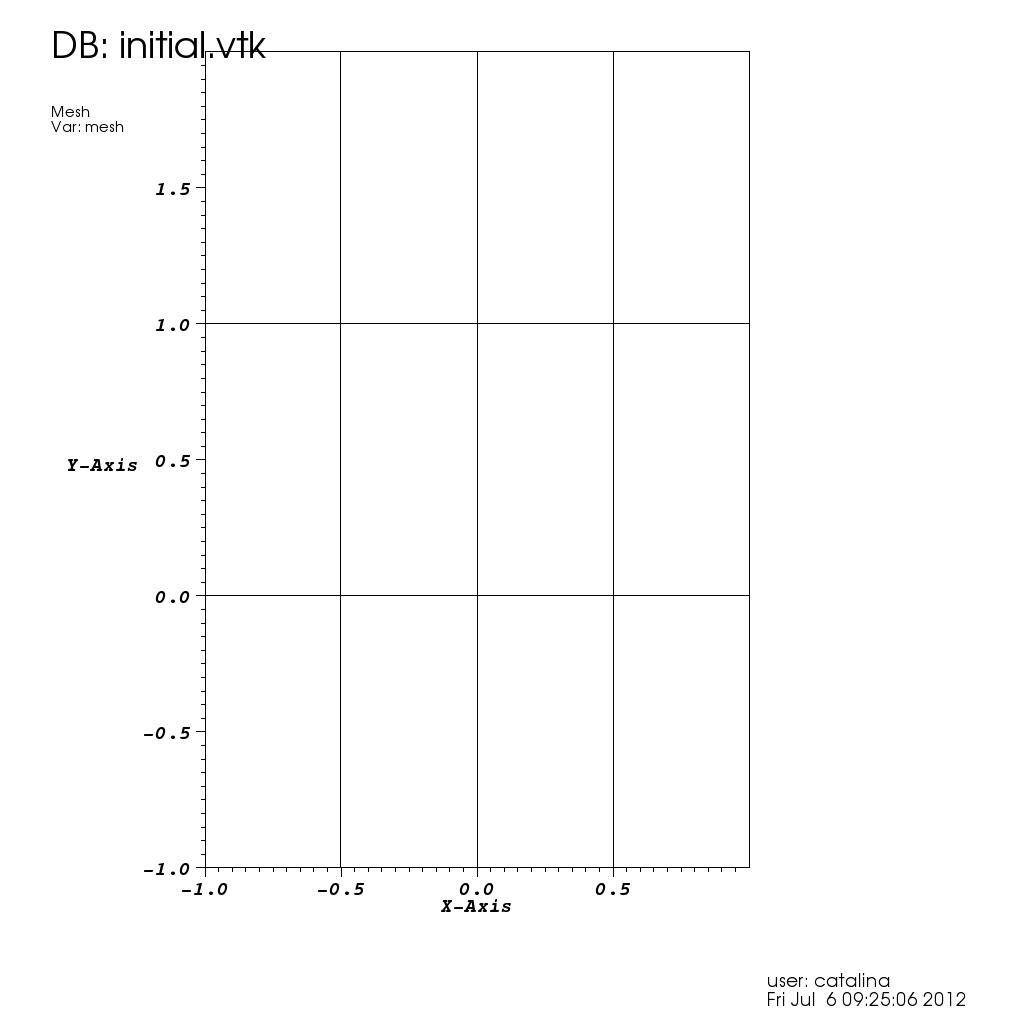
\includegraphics[height=4.5cm,width=4.5cm]{figuras/initial0001.png}



\vspace{0.3cm}
\textbf{Fazer refinamentos e níveis}
\begin{itemize}
\item Dividir em 2 dir X e dir Y da célula que contem o ponto $P(0,0)$
\begin{verbatim}
Point p;
p[0] = 0.0;
p[1] = 0.0;
hig_cell *c =
   hig_get_cell_with_point(root,p);
num_cells[0] = 2;
num_cells[1] = 2;
hig_refine_uniform(c,num_cells);
\end{verbatim}
\end{itemize}
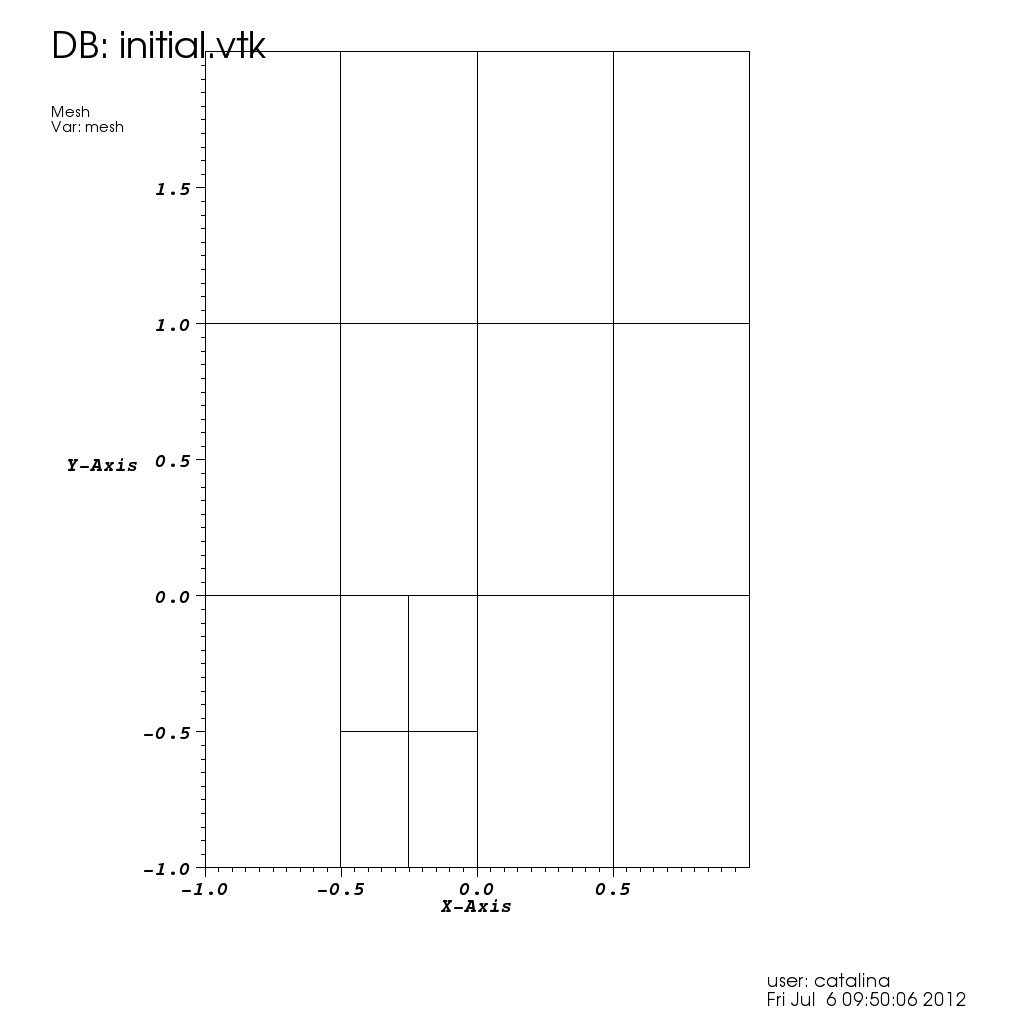
\includegraphics[height=4cm,width=4cm]{figuras/initial0002.png}


\begin{itemize}
\item Refinar consecutivamente ao redor de um ponto
\begin{verbatim}
for (int i = 0; i < 5; i++){
  c = hig_get_cell_with_point(root,p);
  hig_refine_uniform(c,num_cells);
}
\end{verbatim}
\end{itemize}
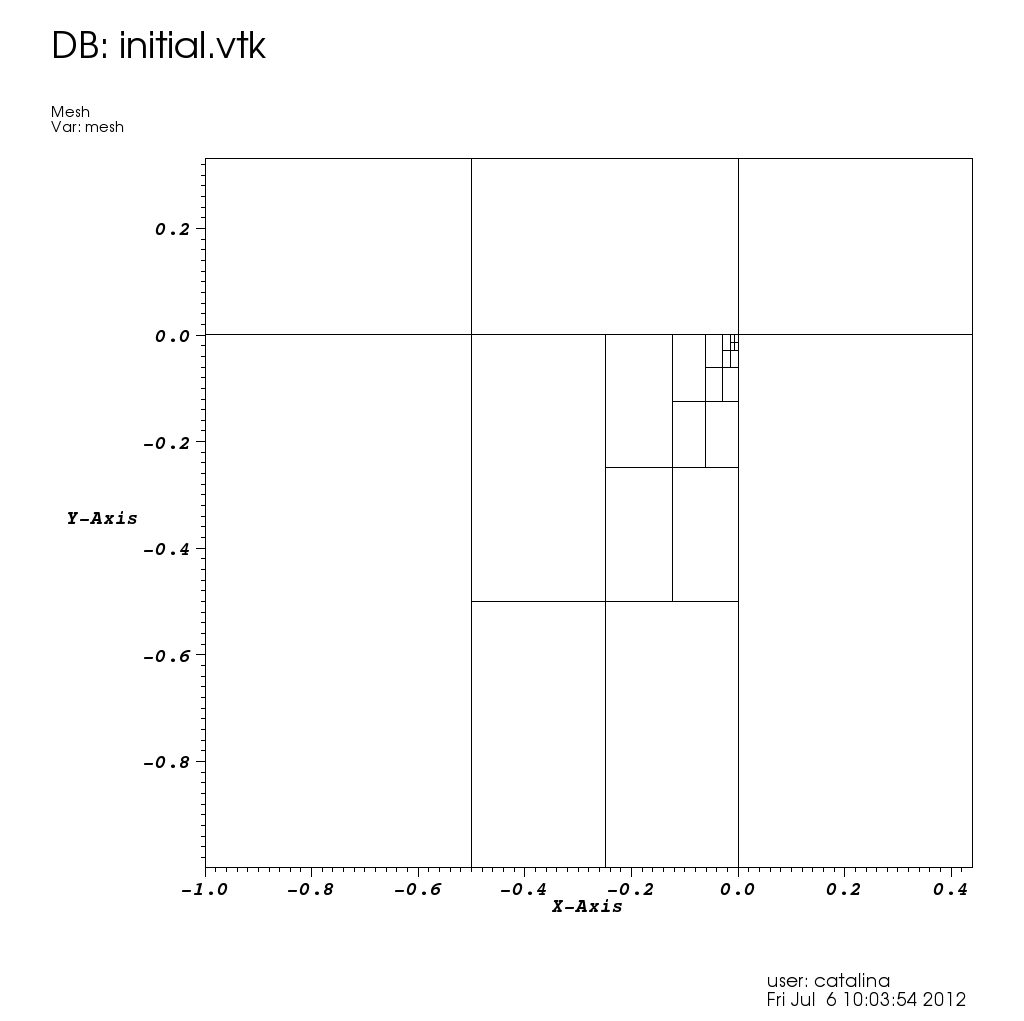
\includegraphics[height=4cm,width=4cm]{figuras/initial0004.png}
\vspace{0.2cm}
\textbf{Refinamento em pontos aleatórios}
\vspace{-0.2cm}
\begin{verbatim}
   for(int j = 0; j < 10; j++){
     p[0] = 2.0*((double)rand()/(double)RAND_MAX)-1.0;
     p[1] = 2.0*((double)rand()/(double)RAND_MAX)-1.0;
     for (int i = 0; i < 5; i++){
        c = hig_get_cell_with_point(root,p);
        hig_refine_uniform(c,num_cells);
     }
   }
\end{verbatim}



\begin{itemize}
\item Refinamento escolhendo na mão a célula para refinar
\begin{verbatim}
hig_cell *c = hig_get_child(root,4);
num_cells[0] = 5;
num_cells[1] = 5;
hig_refine_uniform(c,num_cells);
\end{verbatim}
\end{itemize}
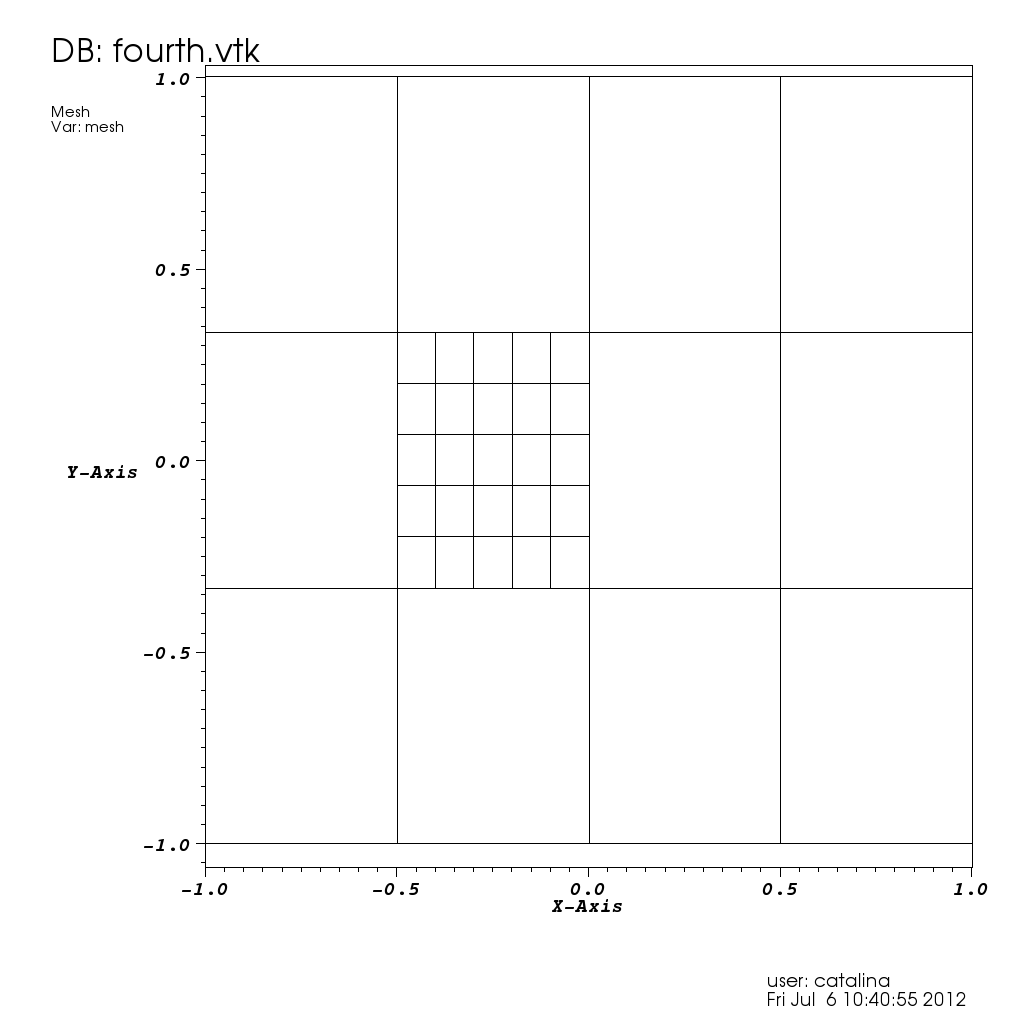
\includegraphics[height=4cm,width=4cm]{figuras/initial0005.png}

\bf{Exercício}
\begin{figure}[htbp]
\centering
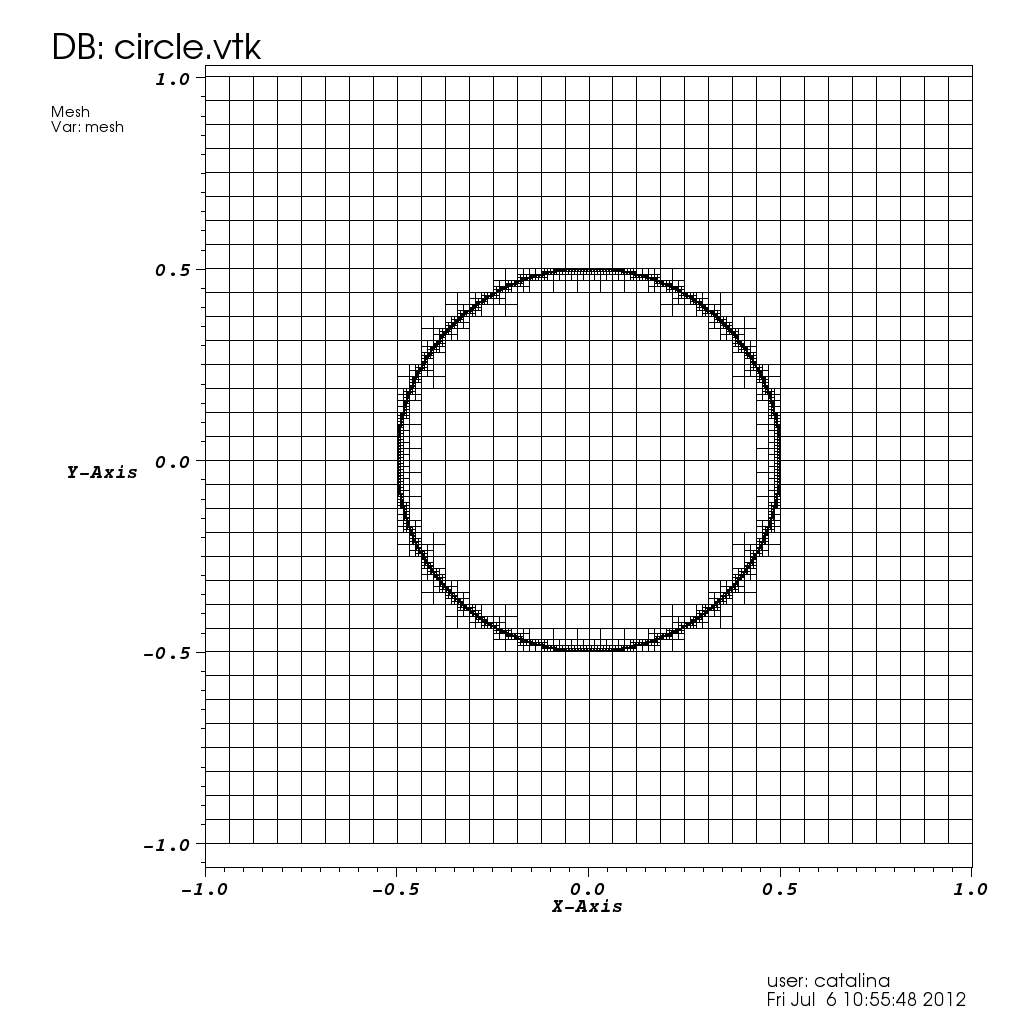
\includegraphics[height=6cm,width=6cm]{figuras/initial0006.png}
\end{figure}



%%%%%%%%%%%%%%%%%%%%%%%%%%%%%%%%%%%%%%%%%%%%%%%%%%%%%%%%%%%%%%%%%%%%%%%%%%%%%%%
\section{Parte III}

\bf{Malhas com estrutura m-tree: atividade da semana III}

Vamos *gerar* na mão uma m-tree e repetir o exercício da curva da semana anterior.
